\documentclass[conference]{IEEEtran}
\IEEEoverridecommandlockouts
% The preceding line is only needed to identify funding in the first footnote. If that is unneeded, please comment it out.
\usepackage{cite}
\usepackage{amsmath,amssymb,amsfonts}
\usepackage{algorithm}
\usepackage{algorithmic}
\usepackage{graphicx}
\usepackage{textcomp}
\usepackage{xcolor}
\usepackage{float}
\usepackage[section]{placeins} % chặn float vượt khỏi section/subsection
\usepackage{url}
\usepackage{tikz}
\usepackage{multirow}
\usepackage{caption}
\usepackage{cuted} % provides strip environment
\usetikzlibrary{positioning,arrows.meta,shapes.geometric}

\def\BibTeX{{\rm B\kern-.05em{\sc i\kern-.025em b}\kern-.08em
    T\kern-.1667em\lower.7ex\hbox{E}\kern-.125emX}}
\begin{document}

% ================= Title =======================
\title{Dual-Perspective Deepfake Detection via Forensic–Physiological Temporal Fusion.\\
% {\footnotesize \textsuperscript{*}Note: Sub-titles are not captured in Xplore and
% should not be used}
}

% ================= Author =======================
% \author{\IEEEauthorblockN{1\textsuperscript{st} Quang Dang Huu}
% \IEEEauthorblockA{\textit{dept. name of organization (of Aff.)} \\
% \textit{name of organization (of Aff.)}\\
% City, Country \\
% email address or ORCID}
% \and
% \IEEEauthorblockN{2\textsuperscript{nd} Tien Tran Thi Mi}
% \IEEEauthorblockA{\textit{dept. name of organization (of Aff.)} \\
% \textit{name of organization (of Aff.)}\\
% City, Country \\
% email address or ORCID}
% \and
% \IEEEauthorblockN{3\textsuperscript{rd} Given Name Surname}
% \IEEEauthorblockA{\textit{dept. name of organization (of Aff.)} \\
% \textit{name of organization (of Aff.)}\\
% City, Country \\
% email address or ORCID}
% \and
% \IEEEauthorblockN{4\textsuperscript{th} Given Name Surname}
% \IEEEauthorblockA{\textit{dept. name of organization (of Aff.)} \\
% \textit{name of organization (of Aff.)}\\
% City, Country \\
% email address or ORCID}
% \and
% \IEEEauthorblockN{5\textsuperscript{th} Given Name Surname}
% \IEEEauthorblockA{\textit{dept. name of organization (of Aff.)} \\
% \textit{name of organization (of Aff.)}\\
% City, Country \\
% email address or ORCID}
% \and
% \IEEEauthorblockN{6\textsuperscript{th} Given Name Surname}
% \IEEEauthorblockA{\textit{dept. name of organization (of Aff.)} \\
% \textit{name of organization (of Aff.)}\\
% City, Country \\
% email address or ORCID}
% }

\author{
\IEEEauthorblockN{
Dang Huu Quang\textsuperscript{1,2},
Tran Thi Mi Tien\textsuperscript{1,2},
Nguyen Minh Nhut\textsuperscript{1,2} and
Nguyen Dinh Thuan\textsuperscript{1,2}
}
\IEEEauthorblockA{
\textsuperscript{1}University of Information Technology, Ho Chi Minh City, Vietnam \\
\textsuperscript{2}Vietnam National University, Ho Chi Minh City, Vietnam \\
21522508@gm.uit.edu.vn, 21522674@gm.uit.edu.vn, nhutnm.17@grad.uit.edu.vn, thuannd@uit.edu.vn
}}

\maketitle

% ================= Abstraction =======================
\begin{abstract}
The rapid advancement of deepfake technology poses significant risks to biometric security systems, particularly in mobile banking applications that rely on face authentication. As synthetic facial media becomes increasingly realistic, existing detection methods that depend on a single modality—such as spatial or low-level visual cues—often exhibit limited robustness under real-world mobile capture conditions. To address this challenge, this paper proposes a dual-perspective deepfake detection framework that jointly leverages frequency-domain forensics and behavioral signal analysis. The frequency-domain module exploits Fast Fourier Transform (FFT), Discrete Cosine Transform (DCT), and Spatial Rich Model (SRM) residuals to uncover abnormal noise patterns and compression-induced artifacts introduced during facial manipulation, while the behavioral analysis module captures physiological and motion-consistency cues, including natural blinking rhythms, gaze dynamics, and head-pose coherence, which remain challenging for generative models to reproduce reliably. Experimental results demonstrate that integrating these two types of evidence improves robustness against increasingly sophisticated deepfake attacks, indicating the potential of the proposed approach for future face-authentication and synthetic media forensics systems.
\end{abstract}

\begin{IEEEkeywords}
Deepfake detection, frequency domain analysis, FFT, DCT, Spatial Rich Model (SRM), forensic traces, behavioral cues, blink analysis, eye-tracking, head-pose estimation, synthetic media forensics.
\end{IEEEkeywords}


% ================= I. Introduction =======================
% \section{Introduction}
% % Raw content
% Deepfake generation has advanced rapidly, raising practical risks for biometric security systems that rely on face verification. As modern generators improve visual quality and temporal coherence, detectors that rely on a single family of cues (purely spatial textures or a single artifact type) become less reliable under compression, post-processing, and cross-dataset deployment.

% We therefore focus on a hybrid perspective that combines (i) forensic traces that can be emphasized in the frequency/residual domain and (ii) behavioral signals that capture how faces move over time. Frequency-domain representations (e.g., FFT and DCT statistics) and residual modeling (e.g., SRM-style high-pass responses) can highlight subtle synthesis and compression inconsistencies that are hard to notice in RGB space~\cite{b9,b19}. Complementarily, physiological and motion-related cues such as blinking dynamics and head pose consistency provide an additional channel that is difficult for generators to reproduce perfectly~\cite{b10,b11}.

% Motivated by these two complementary sources of evidence, we propose a dual-stream deepfake detection framework for mobile banking-style face authentication scenarios. Spatial facial frames are encoded by a lightweight CNN backbone (MobileNetV2)~\cite{b17} while a parallel stream aggregates frequency/forensic and behavioral descriptors, including OpenFace-based signals~\cite{b18}. These streams are fused and modeled temporally using three alternative architectures (BiGRU+attention, BiLSTM+attention+KAN, and TCN with residual blocks). We propose a dual-stream deepfake detector that fuses features, benchmark three temporal backbones (BiGRU, BiLSTM+KAN, TCN), and validate on FaceForensics++ and Celeb-DF with cross-validation and HMM smoothing.

% ================= I. Introduction =======================
\section{Introduction}

The rapid advancement of deepfake technology poses significant risks to biometric security systems, particularly in mobile banking applications that rely on face authentication. Modern generative models produce highly realistic facial videos with improved visual quality and temporal coherence, making traditional detectors that rely on a single modality—such as spatial textures or a specific artifact type—less reliable under video compression, post-processing, and cross-dataset deployment~\cite{b1,b2,b5}.

Frequency-domain representations (e.g., FFT, DCT, SRM residuals) can reveal subtle synthesis and compression inconsistencies, but are often sensitive to device-specific noise and diverse capture conditions~\cite{b5,b9}. In contrast, behavioral signals—such as blinking dynamics, gaze direction, and head-pose consistency—provide complementary information that generative models struggle to reproduce accurately. However, these signals can be limited by temporal discontinuities and user variability, particularly in short mobile authentication sessions~\cite{b6,b10,b11}. Current single-modality detectors fail to fully exploit the synergy of these complementary cues, motivating the development of a hybrid detection approach.

In this work, we propose a dual-stream deepfake detection framework for mobile banking-style face authentication. The framework simultaneously leverages (i) \emph{frequency-domain forensic features} extracted from facial frames using FFT, DCT, and SRM residuals, and (ii) \emph{behavioral features} captured via OpenFace~\cite{b18}, including blinking dynamics, gaze direction, and head-pose consistency. Spatial facial frames are encoded using a lightweight CNN backbone, MobileNetV2~\cite{b17}, while the two streams are fused and temporally modeled using three alternative architectures: BiGRU with attention, BiLSTM with attention and KAN, and Temporal Convolutional Networks (TCN) with residual blocks. This design captures both short-term and long-term temporal dependencies while remaining efficient for mobile deployment.

We evaluate the proposed framework on the \emph{FaceForensics++}~\cite{b8,b13} and \emph{Celeb-DF}~\cite{b14} datasets, employing cross-validation and HMM-based temporal smoothing to improve robustness. By integrating frequency and behavioral cues, the framework addresses the limitations of single-domain detectors and enhances the reliability of face authentication in real-world mobile banking scenarios.


% % ================= II. Related work =======================
% \section{Related work}
% % \subsection{Maintaining the Integrity of the Specifications}
% % Raw content
% A large body of work has explored deepfake detection from multiple angles, ranging from visual artifacts to behavioral signals. Afchar \textit{et al.} introduced MesoNet, a compact CNN designed to capture manipulation artifacts under compression~\cite{b1}. Public benchmarks such as Celeb-DF have helped evaluate detector robustness on higher-quality forgeries and highlight generalization gaps~\cite{b2,b14}.

% Beyond purely spatial artifact analysis, several studies emphasize complementary signals. Behavioral and physiological inconsistencies (e.g., abnormal blinking) have been used as discriminative cues for forged videos~\cite{b10}. Inconsistent 3D head pose trajectories also provide evidence of manipulation when synthesis pipelines fail to preserve geometry over time~\cite{b11}. Recent hybrid approaches further show that combining appearance with eye-related signals can improve detection robustness in practice~\cite{b6}.

% On the forensic side, frequency- and residual-based approaches aim to expose subtle traces that may not be visually salient. DCT-domain anomalies can capture quantization and generation artifacts~\cite{b9}, while camera-model fingerprints such as Noiseprint support manipulation analysis via residual patterns~\cite{b4}. Frequency-aware deepfake detectors have also been proposed to improve generalization across unseen generators~\cite{b5}.

% In this work, we combine frequency/forensic descriptors (FFT, DCT, SRM-style residual statistics) with behavioral signals (OpenFace) and model temporal dynamics using multiple sequence backbones. This hybrid design is motivated by the observation that different deepfake generation pipelines fail in different ways: some leave stronger forensic traces, while others are better exposed through temporal-behavioral inconsistencies.

% ================= II. Related Work =======================
\section{Related Work}

Deepfake detection has evolved from analyzing single-frame artifacts to modeling complex temporal and behavioral inconsistencies. We categorize existing approaches into three main streams: spatial-artifact detection, behavioral analysis, and frequency-domain forensics.

\subsection{Spatial and Artifact-based Detection}
Early methods focused on identifying visual anomalies introduced by the upsampling steps in autoencoder-based generation. Afchar et al.~\cite{b1} proposed MesoNet, a lightweight CNN designed to capture mesoscopic properties of image forgeries. Similarly, other CNN-based approaches leverage standard backbones, such as MobileNetV2~\cite{b17} or Xception, to extract frame-level features. While these methods are effective on low-quality deepfakes, they often struggle to generalize across different generation methods and suffer from performance degradation when facing high-quality forgeries or video compression, as highlighted by benchmarks like FaceForensics++~\cite{b8} and Celeb-DF~\cite{b2,b14}.

\subsection{Behavioral and Physiological Analysis}
To overcome the limitations of spatial features, researchers have explored high-level semantic cues that generative models struggle to replicate. Li et al.~\cite{b10} utilized the frequency of eye blinking to expose deepfakes, as early generation algorithms often produced faces with permanently open eyes due to biased training data. Yang et al.~\cite{b11} exploited inconsistencies in 3D head poses, while Qi et al.~\cite{b3} analyzed biological signals, specifically detecting synthetic videos via heart rate estimation (DeepRhythm). Recently, hybrid approaches~\cite{b6} have begun combining eye-movement analysis with deep learning features. Although behavioral signals are robust to visual compression, they require temporal continuity and can be less effective in short video clips where specific behaviors (e.g., blinking) may not occur naturally.

\subsection{Frequency-domain and Forensic Analysis}
Since spatial artifacts can be masked by post-processing, frequency-domain analysis aims to uncover invisible traces. Methods based on the Discrete Cosine Transform (DCT)~\cite{b9} and Fast Fourier Transform (FFT) typically reveal abnormal spectral distributions caused by upsampling operations. Furthermore, camera-based fingerprints, such as Noiseprint~\cite{b4} and PRNU~\cite{b7}, have been adapted to detect inconsistencies between the facial region and the background. Fridrich et al.~\cite{b19} introduced the Spatial Rich Model (SRM), originally for steganalysis, which has proven effective in isolating residual noise patterns in deepfakes. Recent work like FreqNet~\cite{b5} demonstrates that frequency-aware detectors significantly improve cross-generator generalization.

\subsection{Our Approach}
Existing methods often rely on a single modality, making them vulnerable when that specific trace is removed or improved by newer generators. Motivated by this, our framework proposes a dual-perspective fusion. We utilize MobileNetV2~\cite{b17} for efficient spatial feature extraction and integrate SRM~\cite{b19} and frequency analysis to capture micro-level artifacts. Simultaneously, we employ OpenFace~\cite{b18} to extract robust behavioral signals. Unlike static approaches, we model the temporal evolution of these features using sequence models smoothed by Hidden Markov Models (HMM)~\cite{b20}, thereby combining the precision of forensic analysis with the semantic robustness of behavioral cues.


% Raw content

% ================ III. Methodologies 1=======================
% \section{Methodologies}

% This section describes the overall framework for deepfake detection, including data preprocessing, frequency-domain analysis, behavioral feature extraction, fusion strategy, and training configuration. An overview of the proposed pipeline is shown in Fig.~\ref{fig:pipeline}.
% \begin{figure}[htbp]
% \centering
% \begin{tikzpicture}[
%     node distance=4mm and 6mm,
%     box/.style={draw, rounded corners, align=center, inner sep=4pt, minimum height=7mm},
%     arrow/.style={-Latex, thick}
% ]
% \node[box] (video) {Input video\\(cropped face frames)};
% \node[box, below=of video] (seq) {Sequence formation\\($T$ frames + padding)};

% \node[box, below left=of seq, xshift=5mm] (imgprep) {Resize $224\times224$\\Normalize $[0,1]$\\Augment (train)};
% \node[box, below right=of seq, xshift=-5mm] (feat) {Per-frame\\ fused features\\FFT + DCT +\\ SRM + OpenFace};

% \node[box, below=of imgprep] (cnn) {MobileNetV2\\frame embeddings};
% \node[box, below=of feat] (scaler) {StandardScaler\\(fit on train)};

% \node[box, below=of seq, yshift=-36mm] (fusion) {Late fusion\\(concat embeddings + features)};
% \node[box, below=of fusion] (temporal) {Temporal model\\BiGRU / BiLSTM+KAN / TCN};
% \node[box, below=of temporal] (hmm) {HMM smoothing\\(post-processing)};
% \node[box, below=of hmm] (out) {Video-level label};

% \draw[arrow] (video) -- (seq);
% \draw[arrow] (seq) -- (imgprep);
% \draw[arrow] (seq) -- (feat);
% \draw[arrow] (imgprep) -- (cnn);
% \draw[arrow] (feat) -- (scaler);
% \draw[arrow] (cnn) -- (fusion);
% \draw[arrow] (scaler) -- (fusion);
% \draw[arrow] (fusion) -- (temporal);
% \draw[arrow] (temporal) -- (hmm);
% \draw[arrow] (hmm) -- (out);
% \end{tikzpicture}
% \caption{Overview of the proposed deepfake detection pipeline.}
% \label{fig:pipeline}
% \end{figure}
% % ------------- 3.1 Overview --------------
% % \subsection{Overview}
% % % TODO: Describe the system pipeline, dual-branch architecture (frequency + behavioral), overall workflow, and figure reference.
% % \begin{figure}[htbp]
% % \centerline{\includegraphics[width=0.48\textwidth]{pipeline.png}}
% % \caption{Overview of the proposed dual-branch deepfake detection framework combining frequency-domain analysis and behavioral feature extraction.}
% % \label{fig:pipeline}
% % \end{figure}

% % ------------- 3.2 Pre-processing --------------
% \subsection{Pre-processing}

% The preprocessing pipeline transforms raw video data into structured sequences suitable for dual-branch feature extraction. The process consists of five main stages: frame extraction and parsing, face detection and cropping, sequence formation, feature extraction, and normalization.

% \textbf{Frame Extraction and Indexing.} Each video is decomposed into individual frames stored as JPEG images following the naming convention \texttt{videoID\_frameNumber.jpg} (e.g., \texttt{000\_id0\_0000\_frame\_0000.jpg}). The filename encodes both video identity and temporal position, enabling efficient frame-to-video mapping and sequential ordering. A dataframe is constructed to catalog all frames with their corresponding video IDs, frame indices, file paths, and binary labels (fake=0, real=1). Videos are grouped using a unique \texttt{video\_key} identifier combining the video ID and label, creating a dictionary structure that maps each video to its ordered frame sequence.

% \csname textbf\endcsname{Face Crops and Alignment.} We operate on cropped and aligned face regions provided by the dataset preprocessing. This keeps the model focused on the facial area and improves spatial consistency across frames, which is important for both CNN-based appearance modeling and behavioral feature extraction.

% \csname textbf\endcsname{Spatial Normalization.} All face crops are resized to $224 \times 224$ pixels to match the input requirements of MobileNetV2~\cite{b17}. Pixel intensities are normalized to $[0, 1]$ by dividing by 255. During training, we apply data augmentation using Keras ImageDataGenerator. For the BiGRU and BiLSTM-KAN experiments, the augmentation includes random rotation ($\pm 15^\circ$), horizontal flipping, and zoom perturbations ($\pm 10\%$). For the TCN experiments, we use a stronger augmentation that additionally includes width/height shifts ($\pm 15\%$) and brightness changes in the range $[0.8, 1.2]$. No augmentation is applied during validation and testing.

% \csname textbf\endcsname{Temporal Sequence Formation.} Frames belonging to the same video are organized into fixed-length temporal sequences. For BiGRU and BiLSTM-KAN we use $T=10$, while for TCN we use $T=15$ to provide a longer temporal context. Videos with fewer frames than $T$ are padded with zeros, and longer videos are truncated to the first $T$ frames.

% \textbf{Frequency and Behavioral Feature Extraction.} In parallel with spatial frame processing, a comprehensive set of frequency-domain and behavioral features is pre-computed for each frame to capture artifacts invisible to the naked eye. This process involves four distinct extractors:

% \textit{1) FFT-based Frequency Analysis:} Frames are converted to grayscale and resized to $256 \times 256$ pixels. A Hanning window is applied to reduce spectral leakage before computing the 2D Fast Fourier Transform (FFT). We extract the Power Spectral Density (PSD) and Log-PSD, removing the DC component to focus on texture patterns. Key features include band energies (low, mid, high frequencies), radial and angular profiles (averaged over 64 radial and 12 angular bins), spectral flatness, entropy, and specific energy markers at $8 \times 8$ block boundaries to detect JPEG compression inconsistencies.

% \textit{2) DCT-based Artifact Analysis:} The Y-channel (luminance) of the $256 \times 256$ image is divided into non-overlapping $8 \times 8$ blocks. For each block, the 2D Discrete Cosine Transform (DCT-II) is computed. We analyze the log-magnitude of coefficients across three frequency bands: Low ($3 \times 3$ top-left), Mid ($6 \times 6$ excluding Low), and High (remaining coefficients). Statistical moments (mean, variance, skewness, kurtosis), Shannon entropy, and histograms are calculated for each band, along with the first 20 zig-zag coefficients, to capture quantization artifacts typical of deepfake synthesis.

% \csname textit\endcsname{3) Spatial Rich Model (SRM) Features:} We extract SRM-style residual statistics using high-pass filter responses to emphasize local noise inconsistencies that are informative for image forensics~\cite{b19}.

% \csname textit\endcsname{4) Behavioral Signals (OpenFace):} We utilize the OpenFace toolkit~\cite{b18} to extract physiological and behavioral cues, including facial landmarks, head pose, eye gaze, and facial action units (AUs).

% All extracted features (FFT, DCT, SRM, OpenFace) are concatenated into a single high-dimensional vector per frame and stored in a structured CSV format, indexed by filename.

% \textbf{Feature Normalization.} The fused feature vectors are standardized using $z$-score normalization. A StandardScaler is fitted on the training set to compute the mean and standard deviation for each feature dimension. These statistics are then used to normalize the training, validation, and test sets, ensuring zero mean and unit variance. This step is crucial for the convergence of the subsequent neural network layers.

% The final output of the preprocessing stage consists of two synchronized data streams per video sequence: (1) a spatial stream containing $T$ normalized RGB frames of size $224 \times 224 \times 3$, and (2) a frequency-behavioral stream containing $T$ normalized feature vectors of dimension $D$ (where $D$ is the total dimension of the fused features). These dual streams are batched and fed into the corresponding branches of the detection network.
% % ------------- 3.3 Model Architectures --------------
% \subsection{Model Architectures}
% This section presents the three distinct deep learning architectures designed to model the temporal dynamics of the fused feature sequences. Let $X = \{x_1, x_2, \dots, x_T\}$ denote the input sequence, where each $x_t \in \mathbb{R}^{D}$ represents the concatenated spatial and frequency-behavioral feature vector at time step $t$. The goal is to learn a mapping $f: X \to \hat{y} \in [0, 1]$ representing the probability of the video being a deepfake.

% \subsubsection{BiGRU with Multi-Head Self-Attention}
% This model leverages Bidirectional Gated Recurrent Units (BiGRU) to capture sequential dependencies and Multi-Head Attention to identify salient frames.

% \begin{figure}[htbp]
% \centerline{\includegraphics[width=0.5\textwidth]{BiGRUwithMulti-HeadSelf-Attention.png}}
% \caption{Proposed BiGRU architecture with Multi-Head Self-Attention.}
% \label{fig:bigru}
% \end{figure}

% The BiGRU processes the sequence in both forward and backward directions. The hidden state $h_t$ is computed as:
% \begin{equation}
% \begin{aligned}
% z_t &= \sigma(W_z x_t + U_z h_{t-1} + b_z) \\
% r_t &= \sigma(W_r x_t + U_r h_{t-1} + b_r) \\
% \tilde{h}_t &= \tanh(W_h x_t + U_h (r_t \odot h_{t-1}) + b_h) \\
% h_t &= (1 - z_t) \odot h_{t-1} + z_t \odot \tilde{h}_t
% \end{aligned}
% \end{equation}
% where $z_t$ and $r_t$ are the update and reset gates. The output is the concatenation of forward and backward states: $H_t = [\overrightarrow{h_t}; \overleftarrow{h_t}]$.

% To capture global dependencies, we apply Multi-Head Attention (MHA). For a query $Q$, key $K$, and value $V$ derived from $H$, the attention output is:
% \begin{equation}
% \text{Attention}(Q, K, V) = \text{softmax}\left(\frac{QK^T}{\sqrt{d_k}}\right)V
% \end{equation}
% The model employs dual MHA blocks (8 heads and 4 heads) followed by Global Average Pooling and a dense classification head.

% \subsubsection{BiLSTM with Attention and KAN}
% This variant replaces GRUs with Long Short-Term Memory (LSTM) units and utilizes a Kolmogorov-Arnold Network (KAN) for the final classification.

% \begin{figure}[htbp]
% \centerline{\includegraphics[width=0.48\textwidth]{bilstm_kan_architecture.png}}
% \caption{BiLSTM architecture integrated with Attention mechanism and KAN.}
% \label{fig:bilstm}
% \end{figure}


% The BiLSTM outputs a sequence of hidden states $H = \{h_1, \dots, h_T\}$. A standard attention mechanism computes a context vector $c$:
% \begin{equation}
% \begin{aligned}
% u_t &= \tanh(W_w h_t + b_w) \\
% \alpha_t &= \frac{\exp(u_t^T u_w)}{\sum_t \exp(u_t^T u_w)} \\
% c &= \sum_{t=1}^T \alpha_t h_t
% \end{aligned}
% \end{equation}
% where $\alpha_t$ represents the importance of the $t$-th frame.

% The final classification uses a KAN layer, which replaces fixed activation functions with learnable univariate functions $\phi$ on edges:
% \begin{equation}
% \text{KAN}(x) = \sum_{j=1}^{N} \phi_{n,j}(x_j)
% \end{equation}
% This allows the network to learn complex non-linear decision boundaries more efficiently than standard MLPs.

% \subsubsection{TCN with Residual Blocks}
% The Temporal Convolutional Network (TCN) models the sequence using dilated causal convolutions, enabling parallel processing and flexible receptive fields.

% \begin{figure}[htbp]
% \centerline{\includegraphics[width=0.45\textwidth]{tcn_architecture.png}}
% \caption{TCN architecture (a) with dilated residual blocks (b).}
% \label{fig:tcn}
% \end{figure}

% The network consists of a stack of residual blocks. For an input sequence $x$ and a filter $f: \{0, \dots, k-1\} \to \mathbb{R}$, the dilated convolution operation $F$ at element $s$ is defined as:
% \begin{equation}
% F(s) = (x *_d f)(s) = \sum_{i=0}^{k-1} f(i) \cdot x_{s - d \cdot i}
% \end{equation}
% where $d$ is the dilation factor, increasing exponentially ($d=2^i$) with network depth $i$. This ensures that the receptive field covers the entire input sequence history without losing resolution.

% \begin{algorithm}
% \caption{General Training Procedure}
% \begin{algorithmic}[1]
% \REQUIRE Video dataset $V$, Labels $Y$
% \FOR{each video $v \in V$}
%     \STATE Extract frames $f_1, \dots, f_T$
%     \STATE Compute spatial features $S = \text{MobileNet}(f)$
%     \STATE Compute freq/behavioral features $F = \text{Extract}(f)$
%     \STATE Concatenate $X_t = [S_t; F_t]$
% \ENDFOR
% \STATE Initialize Model parameters $\theta$
% \WHILE{not converged}
%     \STATE Sample batch $(X, y)$
%     \STATE Forward pass: $\hat{y} = \text{Model}(X; \theta)$
%     \STATE Compute Loss: $\mathcal{L} = -\sum [y \log \hat{y} + (1-y) \log (1-\hat{y})]$
%     \STATE Backward pass: $\nabla_\theta \mathcal{L}$
%     \STATE Update $\theta \leftarrow \theta - \eta \nabla_\theta \mathcal{L}$
% \ENDWHILE
% \end{algorithmic}
% \end{algorithm}

% % ------------- 3.4 Enhancement and fine-tuning --------------
% \subsection{Enhancement and fine-tuning}
% To improve robustness and generalization, we adopt a practical set of regularization and stabilization techniques consistent with our experimental notebooks.

% \subsubsection{Data Augmentation}
% We apply data augmentation only to the training set (see Table~\ref{tab:training_config} and the Data Augmentation subsection in Experiments). The recurrent models (BiGRU and BiLSTM-KAN) use moderate geometric augmentation (rotation, zoom, and horizontal flip), while the TCN experiments use stronger augmentation including shifts and brightness changes.

% \subsubsection{Regularization and Optimization}
% We use dropout in the temporal and dense layers, batch normalization for both the image and feature streams, early stopping based on validation accuracy, and ReduceLROnPlateau to adapt the learning rate. For the MobileNetV2 branch, we fine-tune only the last 20 layers to balance adaptation and overfitting risk.

% \subsubsection{Temporal Smoothing}
% As a post-processing step, we apply an HMM to the sequence of predicted probabilities to encourage temporal consistency and reduce spurious fluctuations (details in the Implementation Details subsection).




% ================ III. Methodologies =======================
% \section{Methodologies}

% This section describes the overall framework for deepfake detection. As illustrated in the pipeline overview (Fig.~\ref{fig:pipeline}), our approach follows a multi-stage process comprising: (1) Data Preprocessing and Sequence Formation, (2) Dual-stream Feature Extraction (Spatial and Frequency-Behavioral branches), (3) Late Fusion, and (4) Temporal Modeling. The following subsections detail the rationale and implementation of each component.

% \begin{figure}[htbp]
% \centering
% \begin{tikzpicture}[
%     node distance=4mm and 6mm,
%     box/.style={draw, rounded corners, align=center, inner sep=4pt, minimum height=7mm},
%     arrow/.style={-Latex, thick}
% ]
% \node[box] (video) {Input video\\(cropped face frames)};
% \node[box, below=of video] (seq) {Sequence formation\\($T$ frames + padding)};

% \node[box, below left=of seq, xshift=5mm] (imgprep) {Resize $224\times224$\\Normalize $[0,1]$\\Augment (train)};
% \node[box, below right=of seq, xshift=-5mm] (feat) {Per-frame\\ fused features\\FFT + DCT +\\ SRM + OpenFace};

% \node[box, below=of imgprep] (cnn) {MobileNetV2\\frame embeddings};
% \node[box, below=of feat] (scaler) {StandardScaler\\(fit on train)};

% \node[box, below=of seq, yshift=-36mm] (fusion) {Late fusion\\(concat embeddings + features)};
% \node[box, below=of fusion] (temporal) {Temporal model\\BiGRU / BiLSTM+KAN / TCN};
% \node[box, below=of temporal] (hmm) {HMM smoothing\\(post-processing)};
% \node[box, below=of hmm] (out) {Video-level label};

% \draw[arrow] (video) -- (seq);
% \draw[arrow] (seq) -- (imgprep);
% \draw[arrow] (seq) -- (feat);
% \draw[arrow] (imgprep) -- (cnn);
% \draw[arrow] (feat) -- (scaler);
% \draw[arrow] (cnn) -- (fusion);
% \draw[arrow] (scaler) -- (fusion);
% \draw[arrow] (fusion) -- (temporal);
% \draw[arrow] (temporal) -- (hmm);
% \draw[arrow] (hmm) -- (out);
% \end{tikzpicture}
% \caption{Overview of the proposed deepfake detection pipeline. The architecture splits into a spatial branch (left) using MobileNetV2 and a frequency-behavioral branch (right) before late fusion.}
% \label{fig:pipeline}
% \end{figure}

% % ------------- 3.2 Pre-processing --------------
% \subsection{Pre-processing}

% The preprocessing pipeline transforms raw video data into structured sequences suitable for dual-branch feature extraction. This corresponds to the top section of Fig.~\ref{fig:pipeline}.

% \textbf{Frame Extraction and Indexing.} Each video is decomposed into individual frames stored as JPEG images following the naming convention \texttt{videoID\_frameNumber.jpg}. The filename encodes both video identity and temporal position. A dataframe is constructed to catalog all frames, and videos are grouped using a unique \texttt{video\_key} identifier to map each video to its ordered frame sequence.

% \textbf{Face Crops and Alignment.} We operate on cropped and aligned face regions. This focuses the model on the facial area, reducing background noise and improving spatial consistency across frames.

% \textbf{Spatial Normalization (Left Branch in Fig.~\ref{fig:pipeline}).} To prepare inputs for the spatial backbone, all face crops are resized to $224 \times 224$ pixels and normalized to $[0, 1]$. During training, data augmentation (rotation $\pm 15^\circ$, zoom $\pm 10\%$, flips) is applied. For TCN experiments, stronger augmentations (shifts, brightness) are used to enhance robustness against lighting variations.

% \textbf{Frequency and Behavioral Feature Extraction (Right Branch in Fig.~\ref{fig:pipeline}).} To capture artifacts invisible to the naked eye, we implement a parallel extraction branch involving four distinct extractors. The rationale for each is as follows:

% \textit{1) FFT-based Frequency Analysis:} Frames are converted to grayscale and processed via 2D Fast Fourier Transform (FFT). We extract Power Spectral Density (PSD) and Log-PSD.
% \textit{Impact:} Generative models (GANs) often leave distinct periodic footprints in the high-frequency spectrum due to upsampling operations (checkerboard artifacts). By analyzing radial and angular spectral profiles, the model can detect these unnatural patterns that are typically smoothed out in the spatial RGB domain.

% \textit{2) DCT-based Artifact Analysis:} We compute the Discrete Cosine Transform (DCT-II) on $8 \times 8$ blocks and analyze coefficients across Low, Mid, and High frequency bands.
% \textit{Impact:} This component is critical for detecting quantization artifacts. Deepfake synthesis often disrupts the natural statistics of DCT coefficients found in authentic camera sensors, creating "double compression" traces that this feature set exposes.

% \textit{3) Spatial Rich Model (SRM) Features:} We extract SRM-style residual statistics using high-pass filters~\cite{b19}.
% \textit{Impact:} SRM residuals emphasize local noise inconsistencies, helping the model identify regions where the noise distribution of the pasted face does not match the background or surrounding regions.

% \textit{4) Behavioral Signals (OpenFace):} We utilize OpenFace~\cite{b18} to extract physiological cues (gaze, head pose, AUs).
% \textit{Impact:} This addresses the semantic limitations of visual detectors. Deepfakes often fail to maintain temporal coherence in biological signals, such as synchronized blinking or natural head-eye coordination. Including these signals allows the model to flag videos that are visually perfect but behaviorally unnatural.

% \textbf{Feature Normalization and Fusion.} The fused frequency-behavioral vectors are $z$-score normalized. Finally, as shown in the "Late fusion" block of Fig.~\ref{fig:pipeline}, the spatial embeddings from MobileNetV2 and the normalized feature vectors are concatenated to form the input $X_t$ for the temporal models.

% % ------------- 3.3 Model Architectures --------------
% \subsection{Model Architectures}
% This section presents the three distinct deep learning architectures designed to model the temporal dynamics of the fused feature sequences.

% \subsubsection{BiGRU with Multi-Head Self-Attention}
% This model leverages Bidirectional Gated Recurrent Units (BiGRU) to capture sequential dependencies and Multi-Head Attention to identify salient frames.

% \begin{figure}[htbp]
% \centerline{\includegraphics[width=0.5\textwidth]{BiGRUwithMulti-HeadSelf-Attention.png}}
% \caption{Proposed BiGRU architecture with Multi-Head Self-Attention.}
% \label{fig:bigru}
% \end{figure}

% The BiGRU processes the sequence in both forward and backward directions (Eq. 1) to integrate past and future context.
% \begin{equation}
% \begin{aligned}
% z_t &= \sigma(W_z x_t + U_z h_{t-1} + b_z) \\
% r_t &= \sigma(W_r x_t + U_r h_{t-1} + b_r) \\
% \tilde{h}_t &= \tanh(W_h x_t + U_h (r_t \odot h_{t-1}) + b_h) \\
% h_t &= (1 - z_t) \odot h_{t-1} + z_t \odot \tilde{h}_t
% \end{aligned}
% \end{equation}
% where $z_t$ and $r_t$ are the update and reset gates. The output is $H_t = [\overrightarrow{h_t}; \overleftarrow{h_t}]$.

% To capture global dependencies, we apply Multi-Head Attention (MHA):
% \begin{equation}
% \text{Attention}(Q, K, V) = \text{softmax}\left(\frac{QK^T}{\sqrt{d_k}}\right)V
% \end{equation}
% \textit{Rationale \& Impact:} Deepfake artifacts (e.g., a momentary glitch in eye alignment) may only appear in a few specific frames while the rest of the video appears authentic. The MHA mechanism allows the model to assign higher attention weights to these "betraying" frames while ignoring temporally consistent but non-informative frames, significantly improving detection sensitivity compared to simple average pooling.

% \subsubsection{BiLSTM with Attention and KAN}
% This variant replaces GRUs with Long Short-Term Memory (LSTM) units and utilizes a Kolmogorov-Arnold Network (KAN) for the final classification.

% \begin{figure}[htbp]
% \centerline{\includegraphics[width=0.48\textwidth]{bilstm_kan_architecture.png}}
% \caption{BiLSTM architecture integrated with Attention mechanism and KAN.}
% \label{fig:bilstm}
% \end{figure}


% The BiLSTM outputs a sequence of hidden states $H$. A standard attention mechanism computes a context vector $c$:
% \begin{equation}
% \begin{aligned}
% u_t &= \tanh(W_w h_t + b_w) \\
% \alpha_t &= \frac{\exp(u_t^T u_w)}{\sum_t \exp(u_t^T u_w)} \\
% c &= \sum_{t=1}^T \alpha_t h_t
% \end{aligned}
% \end{equation}

% The final classification uses a KAN layer, which replaces fixed activation functions with learnable univariate functions $\phi$ on edges:
% \begin{equation}
% \text{KAN}(x) = \sum_{j=1}^{N} \phi_{n,j}(x_j)
% \end{equation}
% \textit{Rationale \& Impact:} Unlike standard MLPs which utilize fixed activation functions (e.g., ReLU), KANs learn the activation functions themselves (parametrized as B-splines). This capability enables the network to approximate the highly non-linear and complex decision boundaries required to distinguish high-quality deepfakes from real faces, especially when they lie close to the real data manifold. This results in higher precision and reduced false alarms.

% \subsubsection{TCN with Residual Blocks}
% The Temporal Convolutional Network (TCN) models the sequence using dilated causal convolutions.

% \begin{figure}[htbp]
% \centerline{\includegraphics[width=0.45\textwidth]{tcn_architecture.png}}
% \caption{TCN architecture (a) with dilated residual blocks (b).}
% \label{fig:tcn}
% \end{figure}

% The dilated convolution operation is defined as:
% \begin{equation}
% F(s) = (x *_d f)(s) = \sum_{i=0}^{k-1} f(i) \cdot x_{s - d \cdot i}
% \end{equation}
% where $d$ is the dilation factor, increasing exponentially ($d=2^i$) with network depth $i$.

% \textit{Rationale \& Impact:} The exponential dilation factor allows the TCN to expand its receptive field to cover the entire input sequence history without losing resolution or significantly increasing computational cost. This architecture is particularly beneficial for detecting long-term behavioral inconsistencies—such as unnatural gradual head movements or breathing patterns—that local convolution operations or short-term RNNs might miss.

% \begin{algorithm}
% \caption{General Training Procedure}
% \begin{algorithmic}[1]
% \REQUIRE Video dataset $V$, Labels $Y$
% \FOR{each video $v \in V$}
%     \STATE Extract frames $f_1, \dots, f_T$
%     \STATE Compute spatial features $S = \text{MobileNet}(f)$ (Left Branch)
%     \STATE Compute freq/behavioral features $F = \text{Extract}(f)$ (Right Branch)
%     \STATE Concatenate $X_t = [S_t; F_t]$ (Fusion)
% \ENDFOR
% \STATE Initialize Model parameters $\theta$
% \WHILE{not converged}
%     \STATE Sample batch $(X, y)$
%     \STATE Forward pass: $\hat{y} = \text{Model}(X; \theta)$
%     \STATE Compute Loss: $\mathcal{L} = -\sum [y \log \hat{y} + (1-y) \log (1-\hat{y})]$
%     \STATE Backward pass: $\nabla_\theta \mathcal{L}$
%     \STATE Update $\theta \leftarrow \theta - \eta \nabla_\theta \mathcal{L}$
% \ENDWHILE
% \end{algorithmic}
% \end{algorithm}

\section{Methodologies}

This section describes the overall framework for deepfake detection, including data preprocessing, frequency-domain analysis, behavioral feature extraction, fusion strategy, and training configuration. An overview of the proposed pipeline is shown in Fig.~\ref{fig:pipeline}.


\textbf{Pipeline Components and Design Rationale.} The proposed framework integrates complementary detection modalities through a carefully designed dual-stream architecture. Component (A) accepts cropped facial regions to eliminate background noise and ensure consistent spatial alignment across frames. Component (B) organizes frames into fixed-length sequences, enabling temporal modeling while handling variable-length videos through padding and truncation strategies.

\begin{figure}[H]
\centering
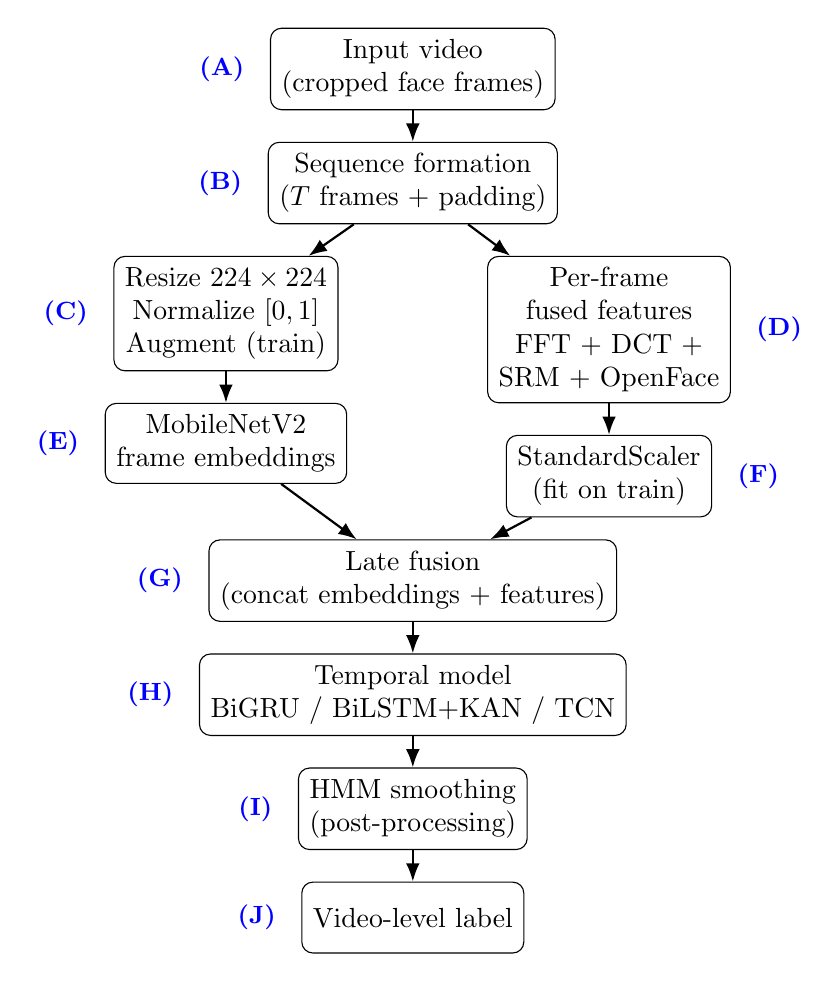
\begin{tikzpicture}[
    node distance=4mm and 6mm,
    box/.style={draw, rounded corners, align=center, inner sep=4pt, minimum height=9mm},
    arrow/.style={-Latex, thick},
    label/.style={font=\small\bfseries, text=blue}
]
\node[box] (video) {Input video\\(cropped face frames)};
\node[label, left=2mm of video] {(A)};

\node[box, below=of video] (seq) {Sequence formation\\($T$ frames + padding)};
\node[label, left=2mm of seq] {(B)};

\node[box, below left=of seq, xshift=15mm] (imgprep) {Resize $224\times224$\\Normalize $[0,1]$\\Augment (train)};
\node[label, left=2mm of imgprep] {(C)};

\node[box, below right=of seq, xshift=-15mm] (feat) {Per-frame\\ fused features\\FFT + DCT +\\ SRM + OpenFace};
\node[label, right=2mm of feat] {(D)};

\node[box, below=of imgprep] (cnn) {MobileNetV2\\frame embeddings};
\node[label, left=2mm of cnn] {(E)};

\node[box, below=of feat] (scaler) {StandardScaler\\(fit on train)};
\node[label, right=2mm of scaler] {(F)};

\node[box, below=of seq, yshift=-36mm] (fusion) {Late fusion\\(concat embeddings + features)};
\node[label, left=2mm of fusion] {(G)};

\node[box, below=of fusion] (temporal) {Temporal model\\BiGRU / BiLSTM+KAN / TCN};
\node[label, left=2mm of temporal] {(H)};

\node[box, below=of temporal] (hmm) {HMM smoothing\\(post-processing)};
\node[label, left=2mm of hmm] {(I)};

\node[box, below=of hmm] (out) {Video-level label};
\node[label, left=2mm of out] {(J)};

\draw[arrow] (video) -- (seq);
\draw[arrow] (seq) -- (imgprep);
\draw[arrow] (seq) -- (feat);
\draw[arrow] (imgprep) -- (cnn);
\draw[arrow] (feat) -- (scaler);
\draw[arrow] (cnn) -- (fusion);
\draw[arrow] (scaler) -- (fusion);
\draw[arrow] (fusion) -- (temporal);
\draw[arrow] (temporal) -- (hmm);
\draw[arrow] (hmm) -- (out);
\end{tikzpicture}
\caption{Overview of the proposed deepfake detection pipeline. The framework consists of dual-stream processing: (A) Input video frames, (B) Temporal sequence formation, (C-E) Spatial branch with MobileNetV2 for appearance modeling, (D-F) Frequency-behavioral branch for forensic and physiological analysis, (G) Late fusion strategy, (H) Temporal modeling, (I) HMM-based post-processing, and (J) Final video-level classification.}
\label{fig:pipeline}
\end{figure}


The architecture then diverges into two parallel branches. The \textit{spatial branch} (C-E) processes RGB frames through MobileNetV2~\cite{b17}, selected for its balance between accuracy and computational efficiency—critical for mobile deployment scenarios. This branch captures high-level semantic features and visible artifacts that distinguish real from synthetic faces. Simultaneously, the \textit{frequency-behavioral branch} (D-F) extracts multi-modal forensic traces that are invisible to spatial detectors. FFT and DCT reveal spectral inconsistencies from GAN upsampling operations~\cite{b5,b9}, SRM residuals expose camera-sensor noise patterns~\cite{b19}, and OpenFace extracts physiological signals (blinking, gaze, head pose) that generative models struggle to replicate coherently~\cite{b10,b11,b18}. This dual-stream design addresses the core limitation of single-modality detectors: when one type of artifact is removed by advanced generators, the complementary stream provides fallback evidence.

Component (G) implements \textit{late fusion}, concatenating the learned spatial embeddings with normalized forensic features. Late fusion is preferred over early fusion because it allows each branch to develop specialized representations before integration—spatial features learn appearance patterns while forensic features remain interpretable. This design also facilitates ablation studies and modular updates.

The fused representations are fed into temporal models (H): BiGRU with multi-head attention, BiLSTM with KAN-based classification, or TCN with dilated convolutions. These architectures capture different aspects of temporal coherence: BiGRU/BiLSTM excel at modeling long-range dependencies critical for detecting subtle frame-to-frame inconsistencies, while TCN provides parallel processing and adjustable receptive fields through exponentially increasing dilation factors~\cite{b5}. Finally, HMM smoothing (I) reduces frame-level prediction noise by enforcing temporal consistency constraints, producing stable video-level decisions (J).

This end-to-end framework is designed to be robust against multiple attack vectors: spatial artifacts, frequency-domain traces, and behavioral inconsistencies. By requiring attackers to simultaneously fool all detection streams, the system significantly raises the bar for successful deepfake generation.

% ------------- 3.2 Pre-processing --------------
\begin{algorithm}[H]
\caption{General Training Procedure}
\begin{algorithmic}[1]
\REQUIRE Video dataset $V$, Labels $Y$
\FOR{each video $v \in V$}
    \STATE Extract frames $f_1, \dots, f_T$
    \STATE Compute spatial features $S = \text{MobileNet}(f)$
    \STATE Compute freq/behavioral features $F = \text{Extract}(f)$
    \STATE Concatenate $X_t = [S_t; F_t]$
\ENDFOR
\STATE Initialize Model parameters $\theta$
\WHILE{not converged}
    \STATE Sample batch $(X, y)$
    \STATE Forward pass: $\hat{y} = \text{Model}(X; \theta)$
    \STATE Compute Loss: $\mathcal{L} = -\sum [y \log \hat{y} + (1-y) \log (1-\hat{y})]$
    \STATE Backward pass: $\nabla_\theta \mathcal{L}$
    \STATE Update $\theta \leftarrow \theta - \eta \nabla_\theta \mathcal{L}$
\ENDWHILE
\end{algorithmic}
\end{algorithm}
\subsection{Pre-processing}

The preprocessing pipeline transforms raw video data into structured sequences suitable for dual-branch feature extraction. The process consists of five main stages: frame extraction and parsing, face detection and cropping, sequence formation, feature extraction, and normalization.

\textbf{Frame Extraction and Indexing.} Each video is decomposed into individual frames stored as JPEG images following the naming convention \texttt{videoID\_frameNumber.jpg} (e.g., \texttt{000\_id0\_0000\_frame\_0000.jpg}). The filename encodes both video identity and temporal position, enabling efficient frame-to-video mapping and sequential ordering. A dataframe is constructed to catalog all frames with their corresponding video IDs, frame indices, file paths, and binary labels (fake=0, real=1). Videos are grouped using a unique \texttt{video\_key} identifier combining the video ID and label, creating a dictionary structure that maps each video to its ordered frame sequence.

\textbf{Face Crops and Alignment.} We operate on cropped and aligned face regions provided by the dataset preprocessing. This keeps the model focused on the facial area and improves spatial consistency across frames, which is important for both CNN-based appearance modeling and behavioral feature extraction. \textit{Rationale:} Background regions introduce irrelevant variations (e.g., different environments, lighting conditions) that reduce model focus on facial manipulation artifacts. Alignment ensures that facial landmarks occupy consistent positions across frames, which is essential for accurate OpenFace feature extraction and inter-frame behavioral consistency analysis.

\textbf{Spatial Normalization.} All face crops are resized to $224 \times 224$ pixels to match the input requirements of MobileNetV2~\cite{b17}. Pixel intensities are normalized to $[0, 1]$ by dividing by 255. During training, we apply data augmentation using Keras ImageDataGenerator. For the BiGRU and BiLSTM-KAN experiments, the augmentation includes random rotation ($\pm 15^\circ$), horizontal flipping, and zoom perturbations ($\pm 10\%$). For the TCN experiments, we use a stronger augmentation that additionally includes width/height shifts ($\pm 15\%$) and brightness changes in the range $[0.8, 1.2]$. No augmentation is applied during validation and testing. \textit{Impact:} Augmentation improves generalization by simulating real-world capture variations (head movements, lighting changes) without requiring additional labeled data. The differential augmentation strategy reflects the different inductive biases of the temporal models: TCN's convolutional nature benefits from stronger geometric variations.

\textbf{Temporal Sequence Formation.} Frames belonging to the same video are organized into fixed-length temporal sequences. For BiGRU and BiLSTM-KAN we use $T=10$, while for TCN we use $T=15$ to provide a longer temporal context. Videos with fewer frames than $T$ are padded with zeros, and longer videos are truncated to the first $T$ frames. \textit{Design rationale:} The sequence length represents a trade-off between temporal coverage and computational efficiency. $T=10$ provides sufficient context for BiGRU/BiLSTM to capture behavioral patterns (e.g., a typical blink lasts 3-4 frames at 30fps), while $T=15$ leverages TCN's parallel processing capability and larger receptive field to model longer-term inconsistencies without significantly increasing memory overhead.

\textbf{Frequency and Behavioral Feature Extraction.} In parallel with spatial frame processing, a comprehensive set of frequency-domain and behavioral features is pre-computed for each frame to capture artifacts invisible to the naked eye. This process involves four distinct extractors:

\textit{1) FFT-based Frequency Analysis:} Frames are converted to grayscale and resized to $256 \times 256$ pixels. A Hanning window is applied to reduce spectral leakage before computing the 2D Fast Fourier Transform (FFT). We extract the Power Spectral Density (PSD) and Log-PSD, removing the DC component to focus on texture patterns. Key features include band energies (low, mid, high frequencies), radial and angular profiles (averaged over 64 radial and 12 angular bins), spectral flatness, entropy, and specific energy markers at $8 \times 8$ block boundaries to detect JPEG compression inconsistencies.

\textit{Contribution:} FFT reveals upsampling artifacts from GAN generators—specifically, periodic patterns in the frequency spectrum caused by bilinear interpolation during image synthesis~\cite{b5}. Real camera images exhibit smooth spectral distributions, while deepfakes show anomalous peaks at specific frequencies. By analyzing both global spectral properties (flatness, entropy) and localized patterns (block boundaries, radial profiles), this module detects both GAN-specific artifacts and compression-recompression inconsistencies introduced during video encoding.

\textit{2) DCT-based Artifact Analysis:} The Y-channel (luminance) of the $256 \times 256$ image is divided into non-overlapping $8 \times 8$ blocks. For each block, the 2D Discrete Cosine Transform (DCT-II) is computed. We analyze the log-magnitude of coefficients across three frequency bands: Low ($3 \times 3$ top-left), Mid ($6 \times 6$ excluding Low), and High (remaining coefficients). Statistical moments (mean, variance, skewness, kurtosis), Shannon entropy, and histograms are calculated for each band, along with the first 20 zig-zag coefficients, to capture quantization artifacts typical of deepfake synthesis.

\textit{Contribution:} DCT analysis targets JPEG compression artifacts and quantization noise patterns. Deepfake generators often apply different compression levels to synthesized faces versus real backgrounds, creating detectable discontinuities in DCT coefficient distributions~\cite{b9}. The $8 \times 8$ block size matches standard JPEG encoding, making this analysis particularly sensitive to compression-recompression cycles. Statistical moments capture distribution shapes (skewness reveals asymmetry, kurtosis detects heavy tails), while entropy measures quantify predictability—real images show consistent entropy patterns, whereas manipulated regions exhibit irregular entropy distributions.

\textit{3) Spatial Rich Model (SRM) Features:} We extract SRM-style residual statistics using high-pass filter responses to emphasize local noise inconsistencies that are informative for image forensics~\cite{b19}.

\textit{Contribution:} SRM was originally designed for steganalysis (detecting hidden data in images) but proves highly effective for deepfake detection. High-pass filters remove image content while preserving noise residuals—real camera images have characteristic noise patterns (Photo Response Non-Uniformity, PRNU) that are sensor-specific~\cite{b7}. Synthesized faces lack these authentic noise patterns or exhibit inconsistent noise between facial regions and background, creating detectable statistical anomalies in the residual domain.

\textit{4) Behavioral Signals (OpenFace):} We utilize the OpenFace toolkit~\cite{b18} to extract physiological and behavioral cues, including facial landmarks, head pose (pitch, yaw, roll), eye gaze direction, and facial action units (AUs).

\textit{Contribution:} Generative models prioritize visual realism but struggle with physiological coherence. Eye blinks follow natural rhythms (15-20 per minute) that deepfakes often fail to replicate~\cite{b10}. Gaze direction should correlate with head pose—violations indicate synthetic generation. Head-pose trajectories should exhibit smooth motion continuity; abrupt changes or physically implausible movements reveal frame-level generation artifacts~\cite{b11}. Action Units (AU1: inner brow raiser, AU12: lip corner puller) capture micro-expressions that are difficult to synthesize consistently across frames. By enforcing these physiological constraints, the behavioral module provides orthogonal evidence independent of visual appearance.

All extracted features (FFT, DCT, SRM, OpenFace) are concatenated into a single high-dimensional vector per frame and stored in a structured CSV format, indexed by filename.

\textbf{Feature Normalization.} The fused feature vectors are standardized using $z$-score normalization. A StandardScaler is fitted on the training set to compute the mean and standard deviation for each feature dimension. These statistics are then used to normalize the training, validation, and test sets, ensuring zero mean and unit variance. This step is crucial for the convergence of the subsequent neural network layers. \textit{Impact:} Without normalization, features with large magnitudes (e.g., FFT energy values) would dominate gradient updates, while small-scale features (e.g., gaze angles) would be ignored. Standardization ensures all features contribute equally during training, improving convergence speed and final accuracy.
The final output of the preprocessing stage consists of two synchronized data streams per video sequence: (1) a spatial stream containing $T$ normalized RGB frames of size $224 \times 224 \times 3$, and (2) a frequency-behavioral stream containing $T$ normalized feature vectors of dimension $D$ (where $D$ is the total dimension of the fused features). These dual streams are batched and fed into the corresponding branches of the detection network.

% % ------------- 3.3 Model Architectures --------------
\subsection{Model Architectures}
This section presents the three distinct deep learning architectures designed to model the temporal dynamics of the fused feature sequences. Let $X = \{x_1, x_2, \dots, x_T\}$ denote the input sequence, where each $x_t \in \mathbb{R}^{D}$ represents the concatenated spatial and frequency-behavioral feature vector at time step $t$. The goal is to learn a mapping $f: X \to \hat{y} \in [0, 1]$ representing the probability of the video being a deepfake.
\textit{Motivation for Multiple Architectures:} We evaluate three fundamentally different temporal modeling paradigms to identify the most effective approach for deepfake detection. Recurrent networks (BiGRU, BiLSTM) excel at capturing long-term dependencies through hidden state propagation, making them suitable for detecting gradual behavioral inconsistencies (e.g., irregular blinking patterns). Attention mechanisms focus on the most discriminative frames, useful when deepfake artifacts are sporadic. TCNs leverage parallel processing and hierarchical receptive fields, enabling efficient capture of multi-scale temporal patterns. By comparing these approaches, we provide insights into which temporal modeling strategy is most robust for this task.

\subsubsection{BiGRU with Multi-Head Self-Attention}
This model leverages Bidirectional Gated Recurrent Units (BiGRU) to capture sequential dependencies and Multi-Head Attention to identify salient frames.

\begin{figure}[H]
\centering
\includegraphics[width=0.5\textwidth]{BIGRU_FINAL.jpg}
\caption{Proposed BiGRU architecture with Multi-Head Self-Attention.}
\label{fig:bigru}
\end{figure}

The BiGRU processes the sequence in both forward and backward directions. The hidden state $h_t$ is computed as:
\begin{equation}
\begin{aligned}
z_t &= \sigma(W_z x_t + U_z h_{t-1} + b_z) \\
r_t &= \sigma(W_r x_t + U_r h_{t-1} + b_r) \\
\tilde{h}_t &= \tanh(W_h x_t + U_h (r_t \odot h_{t-1}) + b_h) \\
h_t &= (1 - z_t) \odot h_{t-1} + z_t \odot \tilde{h}_t
\end{aligned}
\end{equation}
where $z_t$ and $r_t$ are the update and reset gates. The output is the concatenation of forward and backward states: $H_t = [\overrightarrow{h_t}; \overleftarrow{h_t}]$.

\textit{Why BiGRU?} Compared to LSTM, GRU has fewer parameters (no separate cell state), reducing overfitting risk on limited training data while maintaining comparable sequence modeling capability. Bidirectionality is essential for deepfake detection: future frames provide context for interpreting current frames (e.g., a suspicious blink is more telling when followed by prolonged eye closure).
To capture global dependencies, we apply Multi-Head Attention (MHA). For a query $Q$, key $K$, and value $V$ derived from $H$, the attention output is:
\begin{equation}
\text{Attention}(Q, K, V) = \text{softmax}\left(\frac{QK^T}{\sqrt{d_k}}\right)V
\end{equation}
The model employs dual MHA blocks (8 heads and 4 heads) followed by Global Average Pooling and a dense classification head.

\textit{Multi-Head Attention Contribution:} While BiGRU captures sequential patterns, not all frames are equally informative. Attention allows the model to focus on frames with strong deepfake indicators (e.g., frames with unnatural gaze-pose misalignment or suspicious frequency patterns). Multiple heads enable the model to attend to different types of artifacts simultaneously—one head might focus on behavioral anomalies while another emphasizes spectral irregularities. The dual-block design (8 heads + 4 heads) provides both fine-grained and coarse-grained attention patterns.

\subsubsection{BiLSTM with Attention and KAN}

This variant replaces GRUs with Long Short-Term Memory (LSTM) units and utilizes a Kolmogorov-Arnold Network (KAN) for the final classification.

\begin{figure}[htbp]
\centerline{\includegraphics[width=0.48\textwidth]{bilstm_kan_architecture.png}}
\caption{BiLSTM architecture integrated with Attention mechanism and KAN.}
\label{fig:bilstm}
\end{figure}

The BiLSTM outputs a sequence of hidden states $H = \{h_1, \dots, h_T\}$. A standard attention mechanism computes a context vector $c$:
\begin{equation}
\begin{aligned}
u_t &= \tanh(W_w h_t + b_w) \\
\alpha_t &= \frac{\exp(u_t^T u_w)}{\sum_t \exp(u_t^T u_w)} \\
c &= \sum_{t=1}^T \alpha_t h_t
\end{aligned}
\end{equation}
where $\alpha_t$ represents the importance of the $t$-th frame.

\textit{Why LSTM?} LSTM's explicit cell state provides better gradient flow for learning very long-term dependencies (e.g., detecting that a person never blinks throughout a 10-frame sequence). The cell state acts as a "conveyor belt" that carries information across many timesteps without degradation, useful for capturing rare but diagnostic events.

The final classification uses a KAN layer, which replaces fixed activation functions with learnable univariate functions $\phi$ on edges:
\begin{equation}
\text{KAN}(x) = \sum_{j=1}^{N} \phi_{n,j}(x_j)
\end{equation}
This allows the network to learn complex non-linear decision boundaries more efficiently than standard MLPs.

\textit{KAN Contribution:} Traditional MLPs use fixed activation functions (ReLU, sigmoid) which may not optimally separate deepfake features in the learned representation space. KAN learns task-specific activation functions using B-splines, enabling the model to discover complex decision boundaries tailored to deepfake detection. For instance, the relationship between "gaze-pose misalignment" and "fakeness probability" may be highly non-linear—KAN can learn this relationship directly rather than approximating it with pre-defined activations. This provides better expressivity with fewer parameters, reducing overfitting.

\subsubsection{TCN with Residual Blocks}

The Temporal Convolutional Network (TCN) models the sequence using dilated causal convolutions, enabling parallel processing and flexible receptive fields.

\begin{figure}[htbp]
\centerline{\includegraphics[width=0.45\textwidth]{tcn_architecture.png}}
\caption{TCN architecture (a) with dilated residual blocks (b).}
\label{fig:tcn}
\end{figure}

The network consists of a stack of residual blocks. For an input sequence $x$ and a filter $f: \{0, \dots, k-1\} \to \mathbb{R}$, the dilated convolution operation $F$ at element $s$ is defined as:
\begin{equation}
F(s) = (x *_d f)(s) = \sum_{i=0}^{k-1} f(i) \cdot x_{s - d \cdot i}
\end{equation}
where $d$ is the dilation factor, increasing exponentially ($d=2^i$) with network depth $i$. This ensures that the receptive field covers the entire input sequence history without losing resolution.

\textit{Why TCN?} Unlike RNNs, TCNs process all timesteps in parallel (similar to standard CNNs), dramatically reducing training time. Dilated convolutions provide an exponentially growing receptive field: a 4-layer TCN with dilation factors [1, 2, 4, 8] can capture dependencies spanning 32 frames using only 3×3 kernels. This hierarchical approach mimics how deepfake artifacts manifest at multiple timescales: local inconsistencies (frame-to-frame jitter), medium-term patterns (unnatural blink periodicity), and long-term anomalies (monotonic head pose).

\textit{Residual Blocks Contribution:} Residual connections enable training very deep networks by providing gradient highways. For deepfake detection, this allows the model to learn hierarchical feature refinement: early layers detect low-level temporal edges (motion boundaries), middle layers capture mid-level patterns (gaze tracking), and deep layers model high-level semantic inconsistencies (behavioral abnormality). Without residual connections, deep TCNs would suffer from vanishing gradients, limiting their depth and expressivity.


\section{Experiments}
%=============================================================================
% A. DATASETS
%=============================================================================
\subsection{Datasets}
We evaluate the proposed framework on two widely recognized benchmarks: \textbf{FaceForensics++ (FF++)}~\cite{b8, b13} and \textbf{Celeb-DF (v2)}~\cite{b14}. To ensure spatial consistency, all video sequences are pre-processed to extract aligned facial frames using the extraction pipelines provided in their respective official repositories.

\subsubsection{FaceForensics++ (FF++)}
This dataset serves as a standard benchmark comprising 1,000 original video sequences manipulated by four state-of-the-art methods: Deepfakes (DF), Face2Face (F2F), FaceSwap (FS), and NeuralTextures (NT). We specifically utilize the \textbf{c23 (High Quality)} version provided by the official dataset, which employs H.264 encoding. This setting preserves essential forensic traces while accurately reflecting the realistic video conditions often encountered in mobile scenarios. For efficient training and evaluation, we constructed a balanced subset containing \textbf{59,811 frames} (29,974 real and 29,837 fake), randomly sampled from the validation and test splits.

\subsubsection{Celeb-DF (v2)}
To assess robustness against high-fidelity forgeries, we employ Celeb-DF (v2). This dataset addresses the limitations of earlier benchmarks by significantly reducing visual artifacts such as temporal flickering and color inconsistencies. It serves as a challenging benchmark to evaluate the model's \textbf{generalization capability} across previously unseen deepfake generation techniques. Our experimental set consists of \textbf{32,375 frames} (16,172 real and 16,203 fake), specifically selected to evaluate detection performance on high-quality synthetic media.


%========================================================================%=============================================================================

% ----------- References -----------
% Add these to your bibliography file (e.g., refs.bib):
%
% @article{fawcett2006,
%   title={An introduction to ROC analysis},
%   author={Fawcett, Tom},
%   journal={Pattern Recognition Letters},
%   year={2006}
% }
%
% @book{goodfellow2016,
%   title={Deep Learning},
%   author={Goodfellow, Ian and Bengio, Yoshua and Courville, Aaron},
%   year={2016},
%   publisher={MIT Press}
% }
%
% @article{saito2015,
%   title={Precision-Recall Plot Is More Informative than ROC Plot for Imbalanced Data},
%   author={Saito, Takuya and Rehmsmeier, Marc},
%   journal={PLOS ONE},
%   year={2015}
% }
%
% @article{sokolova2009,
%   title={A systematic analysis of performance measures for classification tasks},
%   author={Sokolova, Marina and Lapalme, Guy},
%   journal={Information Processing \& Management},
%   year={2009}
% }


%=============================================================================
% B. IMPLEMENTATION DETAILS
%=============================================================================
\subsection{Implementation Details}

This section describes the hardware, software configuration, training hyperparameters, and data preparation strategies employed in our experiments to ensure reproducibility and transparent reporting of our methodology.

% \subsubsection{Hardware and Software Configuration}
% \mbox{}

% All experiments were conducted on a workstation equipped with the following specifications:

% \textbf{Hardware:}
% \begin{itemize}
%     \item \textbf{CPU}: Dell Precision 3580
%     \item \textbf{RAM}: 32GB
%     \item \textbf{Storage}: SSD for fast data loading
% \end{itemize}

% \textbf{Software Environment:}
% \begin{itemize}
%     \item \textbf{Framework}: TensorFlow 2.x with Keras API
%     \item \textbf{Python Version}: Python 3.10.13
%     \item \textbf{CUDA}: CUDA-enabled GPU acceleration
%     \item \textbf{Key Libraries}:
%         \begin{itemize}
%             \item NumPy 1.24+ for numerical operations
%             \item OpenCV 4.8+ for image processing
%             \item Scikit-learn 1.3+ for evaluation metrics and data splitting
%             \item Pandas for data manipulation
%             \item HMMLearn for Hidden Markov Model post-processing
%         \end{itemize}
%     \item \textbf{CNN Backbone}: MobileNetV2 pre-trained on ImageNet
% \end{itemize}
\subsubsection{Hardware and Software Configuration}
All experiments were conducted on a workstation (Dell Precision 3580) equipped with 32GB of RAM and SSD storage to facilitate fast data loading. The software environment is built upon Python 3.10.13 and the TensorFlow 2.x framework with Keras API, utilizing CUDA-enabled GPU acceleration. Key libraries include NumPy ($1.24+$) for numerical operations, OpenCV ($4.8+$) for image processing, Scikit-learn ($1.3+$) for evaluation metrics and data splitting, Pandas for data manipulation, and HMMLearn for Hidden Markov Model post-processing. Furthermore, we employ MobileNetV2 pre-trained on ImageNet as the CNN backbone.

\subsubsection{Training Configuration}
\mbox{}

Table~\ref{tab:training_config} summarizes the hyperparameters used across all three model architectures. While some parameters vary between models to accommodate their architectural differences, the core training strategy remains consistent.

\begin{table}[htbp]
\centering
\caption{Training Configuration}
\label{tab:training_config}
\begin{tabular}{ll} % Đổi thành 2 cột canh trái (l l) nhìn sẽ thẳng hàng hơn
\hline
\textbf{Parameter} & \textbf{Value} \\
\hline
\multicolumn{2}{c}{\textbf{Common Settings}} \\ % Gộp 2 cột làm 1 và canh giữa tiêu đề
\hline
Optimizer & Adamax \\
Learning Rate & $3 \times 10^{-4}$ \\
Loss Function & Binary Cross-Entropy \\
Epochs & 50 \\
Early Stopping Patience & 5 epochs \\
LR Reduction Factor & 0.5 \\
LR Reduction Patience & 3 epochs \\
Minimum Learning Rate & $1 \times 10^{-6}$ \\
\hline
\multicolumn{2}{c}{\textbf{Model-Specific Settings}} \\
\hline
Batch Size (BiGRU, BiLSTM-KAN) & 32 \\
Batch Size (TCN-Residual) & 16 \\
Seq. Length (BiGRU, BiLSTM-KAN) & 10 frames \\
Seq. Length (TCN-Residual) & 15 frames \\
\hline
\multicolumn{2}{c}{\textbf{Backbone Settings}} \\
\hline
CNN Architecture & MobileNetV2 \\
Pre-trained Weights & ImageNet \\
Trainable Layers & Last 20 layers \\
Feature Extraction & GlobalAveragePooling2D \\
\hline
\multicolumn{2}{c}{\textbf{Regularization}} \\
\hline
Dropout Rate & 0.2 -- 0.3 \\
Batch Normalization & Yes \\
Layer Normalization & Yes (attention layers) \\
\hline
\end{tabular}
\end{table}

\textbf{Optimizer Configuration:} We employ \textit{Adamax}, a variant of the Adam optimizer that utilizes the infinity norm ($L_\infty$) rather than the $L_2$ norm for gradient updates. This choice provides superior stability when handling sparse gradients common in video sequence modeling. The learning rate is initialized at $3 \times 10^{-4}$ and dynamically reduced by a factor of $0.5$ whenever the validation loss plateaus for 3 consecutive epochs, with a minimum floor of $1 \times 10^{-6}$.

\textbf{Loss Function:} To optimize the classification objective, we minimize the Binary Cross-Entropy loss, defined as:
\begin{equation}
    \mathcal{L} = -\frac{1}{N}\sum_{i=1}^{N} [y_i \log(\hat{y}_i) + (1-y_i)\log(1-\hat{y}_i)]
\end{equation}
where $y_i \in \{0,1\}$ denotes the ground truth label ($0=$ fake, $1=$ real) and $\hat{y}_i$ represents the predicted probability.

\textbf{Training Callbacks and Early Stopping:} To prevent overfitting and ensure optimal convergence, we utilize three specific Keras callbacks: \textit{ModelCheckpoint} to save the model instance achieving the highest validation accuracy; \textit{EarlyStopping} to halt training if validation accuracy stagnates for 5 consecutive epochs; and \textit{ReduceLROnPlateau} to adjust the learning rate as described above.

\subsubsection{Data Augmentation}
\mbox{}

To enhance model robustness and prevent overfitting, we apply data augmentation exclusively to the training set using the Keras \textit{ImageDataGenerator}. The augmentation strategy is specifically tailored to the architectural requirements of each model to maximize learning efficiency.

For the \textbf{BiGRU and BiLSTM-KAN} models, we employ a \textbf{Standard Augmentation} protocol. This configuration includes random rotation within $\pm 15^{\circ}$, a zoom range of $\pm 10\%$, horizontal flipping with a probability of $0.5$, and pixel normalization to the $[0, 1]$ range.

In contrast, the \textbf{TCN-Residual} model utilizes an \textbf{Enhanced Augmentation} strategy to handle its deeper architecture. This approach applies more aggressive transformations, including random rotations up to $\pm 20^{\circ}$, width and height shifts of $\pm 15\%$, zoom variations of $\pm 15\%$, brightness adjustments in the range $[0.8, 1.2]$, and horizontal flipping.

Regardless of the augmentation strategy, consistent preprocessing is applied across all data splits. All frames are resized to $224 \times 224$ pixels to match the MobileNetV2 input specifications. Crucially, no augmentation is performed during the validation and testing phases to ensure consistent and fair evaluation conditions.

\subsubsection{Data Split Strategy}
\mbox{}

We employ a stratified 5-fold cross-validation strategy to ensure robust and unbiased evaluation. Specifically, the protocol utilizes Stratified K-Fold with $K=5$ and a random seed of 42 to guarantee reproducibility, strictly maintaining the real/fake ratio across all folds.

For each fold, the data is partitioned into three distinct sets: a \textbf{Test Set} comprising 20\% of the total data (held out for final evaluation), and a remaining portion split 90/10 to form the \textbf{Training Set} (72\% of total data) and the \textbf{Validation Set} (8\% of total data). The validation set is explicitly carved out using an additional stratified split to enable hyperparameter tuning and early stopping decisions. This nested splitting strategy ensures that no data leakage occurs between training, validation, and testing phases.

\textbf{Feature Normalization:} All frequency-domain and behavioral features extracted from OpenFace and frequency analysis (FFT, DCT, SRM) are normalized using \textit{StandardScaler}. The scaler is fitted exclusively on the training data from each fold and then applied to validation and test sets to prevent information leakage. This produces features with zero mean and unit variance, facilitating faster convergence during training.

\textbf{Sequence Formation:} Video frames are organized into fixed-length temporal sequences adapted to the model architecture. We define a sequence length of $T=10$ frames for the BiGRU and BiLSTM-KAN models, whereas the TCN-Residual model utilizes a longer context of $T=15$ frames. For videos with fewer frames than the sequence length, zero-padding is applied. For longer videos, the first $T$ frames are selected to maintain consistency across the dataset.

\textbf{HMM Post-Processing:} Following model prediction, we apply a Gaussian HMM with 2 hidden states (diagonal covariance, 100 EM iterations) for temporal smoothing. The HMM is fitted on the predicted probabilities and the hidden-state sequence is decoded for post-processing. In our implementation, the state-to-label mapping is determined by majority voting using the fold's ground-truth labels. This heuristic improves temporal consistency, but it should be interpreted as a post-processing rule rather than an end-to-end learned module.

This comprehensive implementation strategy ensures reproducible results and fair comparison across different model architectures while maintaining rigorous separation between training and evaluation data.
%=============================================================================
% F. MAIN RESULTS
% Note: Add these packages to your preamble:
% \usepackage{float}
% \usepackage{placeins}
%=============================================================================
% \subsection{Main Results}

% This section presents the evaluation results of the three models, including 
% \textit{TCN + Residual Blocks}, \textit{BiLSTM + Attention + KAN}, and 
% \textit{BiGRU + Multi-Head Self-Attention}, on the FaceForensics++ (FF++) and 
% Celeb-DF datasets.

% All experiments were conducted using a 5-fold cross-validation setup to assess 
% the generalization ability and stability of each model.
% The following tables report the fold-wise performance for each model, followed by summary tables that present the averaged results across all folds.
% We use Accuracy, Precision, 
% Recall, F1-score, and AUC as the evaluation metrics to provide a comprehensive 
% comparison.

% %=============================================================================
% \subsubsection{FaceForensics++ Dataset (FF++)}
% %=============================================================================

% \FloatBarrier
% % \paragraph{TCN + Residual Blocks}
% ~
% \begin{table}[!htbp]
% \centering
% \caption{Fold-wise performance of TCN + Residual Blocks on FaceForensics++ (c23)}
% \label{tab:tcn_ff}
% \begin{tabular}{|c|c|c|c|c|c|}
% \hline
% \textbf{Fold} & \textbf{Accuracy} & \textbf{Precision} & \textbf{Recall} & \textbf{F1} & \textbf{AUC} \\
% \hline
% 1 & 0.8450 & 0.7974 & 0.9250 & 0.8565 & 0.9338 \\
% 2 & 0.8600 & 0.8130 & 0.9350 & 0.8698 & 0.9434 \\
% 3 & 0.8100 & 0.7696 & 0.8850 & 0.8233 & 0.9013 \\
% 4 & 0.8525 & 0.7975 & 0.9450 & 0.8650 & 0.9501 \\
% 5 & 0.8375 & 0.7668 & 0.9700 & 0.8565 & 0.9452 \\
% \hline
% \textbf{Mean} & \textbf{0.8410} & \textbf{0.7889} & \textbf{0.9320} & \textbf{0.8542} & \textbf{0.9348} \\
% \hline
% \end{tabular}
% \end{table}
% \FloatBarrier

% \FloatBarrier
% % \paragraph{BiLSTM + Attention + KAN}
% \begin{table}[!htbp]
% \centering
% \caption{Fold-wise performance of BiLSTM + Attention + KAN on FaceForensics++ (c23)}
% \label{tab:bilstm_ff}
% \begin{tabular}{|c|c|c|c|c|c|}
% \hline
% \textbf{Fold} & \textbf{Accuracy} & \textbf{Precision} & \textbf{Recall} & \textbf{F1} & \textbf{AUC} \\
% \hline
% 1 & 0.5000 & 0.0000 & 0.0000 & 0.0000 & 0.9286 \\
% 2 & 0.8550 & 0.8480 & 0.8650 & 0.8564 & 0.9259 \\
% 3 & 1.0000 & 1.0000 & 1.0000 & 1.0000 & 0.8711 \\
% 4 & 0.8800 & 0.9318 & 0.8200 & 0.8723 & 0.9579 \\
% 5 & 0.8975 & 0.8841 & 0.9150 & 0.8993 & 0.8946 \\
% \hline
% \textbf{Mean} & \textbf{0.8265} & \textbf{0.7328} & \textbf{0.7200} & \textbf{0.7256} & \textbf{0.9156} \\
% \hline
% \end{tabular}
% \end{table}
% \FloatBarrier

% \FloatBarrier
% ~
% \begin{table}[!htbp]
% \centering
% \caption{Fold-wise performance of BiGRU + Multi-Head Self-Attention on FaceForensics++ (c23)}
% \label{tab:bigru_ff}
% \begin{tabular}{|c|c|c|c|c|c|}
% \hline
% \textbf{Fold} & \textbf{Accuracy} & \textbf{Precision} & \textbf{Recall} & \textbf{F1} & \textbf{AUC} \\
% \hline
% 1 & 0.8325 & 0.7671 & 0.9550 & 0.8508 & 0.9376 \\
% 2 & 0.8425 & 0.8072 & 0.9000 & 0.8511 & 0.9261 \\
% 3 & 0.8325 & 0.7806 & 0.9250 & 0.8467 & 0.9273 \\
% 4 & 0.8750 & 0.9213 & 0.8200 & 0.8677 & 0.9537 \\
% 5 & 0.8625 & 0.9191 & 0.7950 & 0.8525 & 0.9398 \\
% \hline
% \textbf{Mean} & \textbf{0.8490} & \textbf{0.8391} & \textbf{0.8790} & \textbf{0.8538} & \textbf{0.9369} \\
% \hline
% \end{tabular}
% \end{table}
% \FloatBarrier

% % \paragraph{Pooled Confusion Matrices (FF++)}
% % To provide a class-wise error breakdown, we compute pooled confusion matrices by concatenating predictions from the test split of each fold (after HMM smoothing) and counting true/false positives and negatives at the video level. The tables below provide the reporting format; counts can be filled once pooled predictions are exported from the evaluation runs.

% % \begin{table}[!htbp]
% % \centering
% % \caption{Pooled confusion matrix on FaceForensics++ (TCN + Residual Blocks)}
% % \label{tab:cm_ff_tcn}
% % \begin{tabular}{|c|c|c|}
% % \hline
% %             \csname textbf\endcsname{True\textbackslash Pred} & \textbf{Fake} & \textbf{Real} \\
% % \hline
% %             \csname textbf\endcsname{Fake} & -- & -- \\
% % \hline
% %             \csname textbf\endcsname{Real} & -- & -- \\
% % \hline
% % \end{tabular}
% % \end{table}

% % \begin{table}[!htbp]
% % \centering
% % \caption{Pooled confusion matrix on FaceForensics++ (BiLSTM + Attention + KAN)}
% % \label{tab:cm_ff_bilstm}
% % \begin{tabular}{|c|c|c|}
% % \hline
% %             \csname textbf\endcsname{True\textbackslash Pred} & \textbf{Fake} & \textbf{Real} \\
% % \hline
% %             \csname textbf\endcsname{Fake} & -- & -- \\
% % \hline
% %             \csname textbf\endcsname{Real} & -- & -- \\
% % \hline
% % \end{tabular}
% % \end{table}

% % \begin{table}[!htbp]
% % \centering
% % \caption{Pooled confusion matrix on FaceForensics++ (BiGRU + Multi-Head Self-Attention)}
% % \label{tab:cm_ff_bigru}
% % \begin{tabular}{|c|c|c|}
% % \hline
% %             \csname textbf\endcsname{True\textbackslash Pred} & \textbf{Fake} & \textbf{Real} \\
% % \hline
% %             \csname textbf\endcsname{Fake} & -- & -- \\
% % \hline
% %             \csname textbf\endcsname{Real} & -- & -- \\
% % \hline
% % \end{tabular}
% % \end{table}

% %=============================================================================
% \subsubsection{Celeb-DF Dataset}
% %=============================================================================

% \FloatBarrier
% ~
% \begin{table}[!htbp]
% \centering
% \caption{Fold-wise performance of TCN + Residual Blocks on Celeb-DF}
% \label{tab:tcn_celeb}
% \begin{tabular}{|c|c|c|c|c|c|}
% \hline
% \textbf{Fold} & \textbf{Accuracy} & \textbf{Precision} & \textbf{Recall} & \textbf{F1} & \textbf{AUC} \\
% \hline
% 1 & 0.5115 & 0.5093 & 0.5093 & 0.5093 & 0.5539 \\
% \hline
% 2 & 0.5023 & 0.0000 & 0.0000 & 0.0000 & 0.5765 \\
% \hline
% 3 & 0.7696 & 0.6980 & 0.9541 & 0.8062 & 0.8773 \\
% \hline
% 4 & 0.5023 & 0.5046 & 0.5046 & 0.5046 & 0.8951 \\
% \hline
% 5 & 0.7731 & 0.8315 & 0.6852 & 0.7513 & 0.8267 \\
% \hline
% \hline
% \textbf{Mean} & \textbf{0.6118} & \textbf{0.5087} & \textbf{0.5306} & \textbf{0.5143} & \textbf{0.7459} \\
% \hline
% \end{tabular}
% \end{table}
% \FloatBarrier

% % \paragraph{Pooled Confusion Matrices (Celeb-DF)}
% % We similarly compute pooled confusion matrices on Celeb-DF by aggregating predictions from all test folds (after HMM smoothing) and counting errors at the video level. The tables below provide the reporting format; counts can be filled once pooled predictions are exported from the evaluation runs.

% % \begin{table}[!htbp]
% % \centering
% % \caption{Pooled confusion matrix on Celeb-DF (TCN + Residual Blocks)}
% % \label{tab:cm_celeb_tcn}
% % \begin{tabular}{|c|c|c|}
% % \hline
% %             \csname textbf\endcsname{True\textbackslash Pred} & \textbf{Fake} & \textbf{Real} \\
% % \hline
% %             \csname textbf\endcsname{Fake} & -- & -- \\
% % \hline
% %             \csname textbf\endcsname{Real} & -- & -- \\
% % \hline
% % \end{tabular}
% % \end{table}

% % \begin{table}[!htbp]
% % \centering
% % \caption{Pooled confusion matrix on Celeb-DF (BiLSTM + Attention + KAN)}
% % \label{tab:cm_celeb_bilstm}
% % \begin{tabular}{|c|c|c|}
% % \hline
% %             \csname textbf\endcsname{True\textbackslash Pred} & \textbf{Fake} & \textbf{Real} \\
% % \hline
% %             \csname textbf\endcsname{Fake} & -- & -- \\
% % \hline
% %             \csname textbf\endcsname{Real} & -- & -- \\
% % \hline
% % \end{tabular}
% % \end{table}

% % \begin{table}[!htbp]
% % \centering
% % \caption{Pooled confusion matrix on Celeb-DF (BiGRU + Multi-Head Self-Attention)}
% % \label{tab:cm_celeb_bigru}
% % \begin{tabular}{|c|c|c|}
% % \hline
% %             \csname textbf\endcsname{True\textbackslash Pred} & \textbf{Fake} & \textbf{Real} \\
% % \hline
% %             \csname textbf\endcsname{Fake} & -- & -- \\
% % \hline
% %             \csname textbf\endcsname{Real} & -- & -- \\
% % \hline
% % \end{tabular}
% % \end{table}

% \FloatBarrier
% \begin{table}[!htbp]
% \centering
% \caption{Fold-wise performance of BiLSTM + Attention + KAN on Celeb-DF}
% \label{tab:bilstm_celeb}
% \begin{tabular}{|c|c|c|c|c|c|}
% \hline
% \textbf{Fold} & \textbf{Accuracy} & \textbf{Precision} & \textbf{Recall} & \textbf{F1} & \textbf{AUC} \\
% \hline
% 1 & 0.8111 & 0.8190 & 0.7963 & 0.8075 & 0.8646 \\
% \hline
% 2 & 0.8111 & 0.9351 & 0.6667 & 0.7784 & 0.9177 \\
% \hline
% 3 & 0.8387 & 0.9302 & 0.7339 & 0.8205 & 0.9269 \\
% \hline
% 4 & 0.8111 & 0.8208 & 0.7982 & 0.8093 & 0.8571 \\
% \hline
% 5 & 0.8194 & 0.8966 & 0.7222 & 0.8000 & 0.8897 \\
% \hline
% \hline
% \textbf{Mean} & \textbf{0.8183} & \textbf{0.8803} & \textbf{0.7435} & \textbf{0.8031} & \textbf{0.8912} \\
% \hline
% \end{tabular}
% \end{table}
% \FloatBarrier

% \FloatBarrier
% \begin{table}[!htbp]
% \centering
% \caption{Fold-wise performance of BiGRU + Multi-Head Self-Attention on Celeb-DF}
% \label{tab:bigru_celeb}
% \begin{tabular}{|c|c|c|c|c|c|}
% \hline
% \textbf{Fold} & \textbf{Accuracy} & \textbf{Precision} & \textbf{Recall} & \textbf{F1} & \textbf{AUC} \\
% \hline
% 1 & 0.8203 & 0.8485 & 0.7778 & 0.8116 & 0.9145 \\
% \hline
% 2 & 0.8341 & 0.8913 & 0.7593 & 0.8200 & 0.9112 \\
% \hline
% 3 & 0.8618 & 0.8624 & 0.8624 & 0.8624 & 0.9317 \\
% \hline
% 4 & 0.8894 & 0.9670 & 0.8073 & 0.8800 & 0.9611 \\
% \hline
% 5 & 0.7685 & 0.7042 & 0.9259 & 0.8000 & 0.8742 \\
% \hline
% \hline
% \textbf{Mean} & \textbf{0.8348} & \textbf{0.8547} & \textbf{0.8265} & \textbf{0.8348} & \textbf{0.9186} \\
% \hline
% \end{tabular}
% \end{table}
% \FloatBarrier

% %=============================================================================
% \subsubsection{Summary and Comparison}
% %=============================================================================

% \vspace{0.3cm}

% Tables~\ref{tab:summary_ff} and~\ref{tab:summary_celeb} summarize the comparative performance of all three temporal architectures across both benchmark datasets.

% % \vspace{0.4cm}

% % \renewcommand{\arraystretch}{1.25}

% % ------------------ FF++ TABLE ---------------------
% \begin{table}[H]
% \centering
% \caption{Summary of average performance on FaceForensics++}
% \label{tab:summary_ff}

% \begin{tabular}{|l|c|c|c|}
% \hline
% \textbf{Metric} & \textbf{TCN} & \textbf{BiLSTM-KAN} & \textbf{BiGRU} \\
% \hline
% Accuracy  & 0.8410 & 0.8265 & \textbf{0.8490} \\
% \hline
% Precision & 0.7889 & 0.7328 & \textbf{0.8391} \\
% \hline
% Recall    & \textbf{0.9320} & 0.7200 & 0.8790 \\
% \hline
% F1-Score  & 0.8542 & 0.7256 & \textbf{0.8538} \\
% \hline
% AUC       & 0.9348 & 0.9156 & \textbf{0.9369} \\
% \hline
% \end{tabular}
% \end{table}

% % ---------------------------------------------------

% \vspace{0.2cm}

% On FaceForensics++, BiGRU + Multi-Head Self-Attention achieves the best overall performance with 84.90\% accuracy and 0.9369 AUC, demonstrating superior balance across all metrics. TCN + Residual Blocks achieves the highest recall (93.20\%), while BiLSTM + Attention + KAN shows the weakest stability.

% % \vspace{0.6cm}

% % ------------------ CELEB-DF TABLE ---------------------
% \begin{table}[H]
% \centering
% \caption{Summary of average performance on Celeb-DF}
% \label{tab:summary_celeb}

% \begin{tabular}{|c|c|c|c|}
% \hline
% \textbf{Metric} & \textbf{TCN} & \textbf{BiLSTM-KAN} & \textbf{BiGRU} \\
% \hline
% Accuracy  & 0.6118 & 0.8183 & \textbf{0.8348} \\
% \hline
% Precision & 0.5087 & \textbf{0.8803} & 0.8547 \\
% \hline
% Recall    & 0.5306 & 0.7435 & \textbf{0.8265} \\
% \hline
% F1-Score  & 0.5143 & 0.8031 & \textbf{0.8348} \\
% \hline
% AUC       & 0.7459 & 0.8912 & \textbf{0.9186} \\
% \hline
% \end{tabular}
% \end{table}
% % ---------------------------------------------------


% \vspace{0.3cm}

% On Celeb-DF, the performance landscape shifts significantly. BiGRU maintains strong generalization (83.48\% accuracy, 0.9186 AUC), while TCN fails with severe performance degradation (61.18\% accuracy). BiLSTM + Attention + KAN achieves the highest precision (88.03\%), making it suitable for high-confidence detection scenarios.

% F. MAIN RESULTS
% Note: Add these packages to your preamble:
% \usepackage{float}
% \usepackage{placeins}
%=============================================================================
% \subsection{Main Results}

\subsection{Main Results}
This section presents the comparative evaluation of our three proposed architectures: \textit{TCN-Residual}, \textit{BiLSTM-KAN}, and \textit{BiGRU-Attention}, on the FaceForensics++ (FF++) and Celeb-DF datasets. All experiments were conducted using a stratified 5-fold cross-validation scheme to assess model generalization.

Table~\ref{tab:main_results} summarizes the averaged performance metrics across all folds for both datasets. We utilize Accuracy, Precision, Recall, F1-score, and AUC to provide a comprehensive assessment.



%=============================================================================
% SINGLE CONSOLIDATED TABLE (non-floating, full-width)
%=============================================================================
\begin{strip}
\centering
\captionof{table}{Comparative Experimental Results on FaceForensics++ and Celeb-DF (Averaged over 5 Folds)}
\label{tab:main_results}
\setlength{\tabcolsep}{6pt}
\renewcommand{\arraystretch}{1.2}
\begin{tabular}{l l c c c c c}
\hline
\textbf{Dataset} & \textbf{Model Architecture} & \textbf{Accuracy} & \textbf{Precision} & \textbf{Recall} & \textbf{F1-Score} & \textbf{AUC} \\
\hline
\multirow{3}{*}{\textbf{FaceForensics++}}
& TCN-Residual    & 0.8410 & 0.7889 & \textbf{0.9320} & \textbf{0.8542} & 0.9348 \\
& BiLSTM-KAN       & 0.8265 & 0.7328 & 0.7200          & 0.7256          & 0.9156 \\
& BiGRU-Attention  & \textbf{0.8490} & \textbf{0.8391} & 0.8790 & 0.8538 & \textbf{0.9369} \\
\hline
\multirow{3}{*}{\textbf{Celeb-DF}}
& TCN-Residual    & 0.6118 & 0.5087 & 0.5306          & 0.5143          & 0.7459 \\
& BiLSTM-KAN       & 0.8183 & \textbf{0.8803} & 0.7435 & 0.8031 & 0.8912 \\
& BiGRU-Attention  & \textbf{0.8348} & 0.8547 & \textbf{0.8265} & \textbf{0.8348} & \textbf{0.9186} \\
\hline
\end{tabular}
\end{strip}


\subsubsection{Performance on FaceForensics++}
On the FaceForensics++ benchmark, all three models demonstrate strong capabilities, with AUC scores exceeding 0.91 across the board. The \textbf{BiGRU-Attention} model achieves the best overall performance, securing the highest Accuracy (84.90\%) and AUC (0.9369), indicating a superior balance between precision and recall. 

The \textbf{TCN-Residual} model, while slightly lower in overall accuracy, excels in sensitivity, achieving the highest Recall of 93.20\%. This suggests that the TCN architecture is particularly effective at detecting fake patterns, though it produces more false positives (Precision 78.89\%) compared to the BiGRU approach.

In contrast, the \textbf{BiLSTM-KAN} model shows the weakest stability on this dataset. A detailed fold-wise analysis (omitted from the table for brevity) revealed significant variance, specifically in Fold 1 where the model failed to converge properly, dragging down the average F1-score to 0.7256. This indicates that while promising, the KAN integration may require more careful hyperparameter tuning for stability.

\subsubsection{Performance on Celeb-DF}
The Celeb-DF dataset, known for its higher visual quality and fewer artifacts, presents a more significant challenge. Here, the performance gap between architectures becomes evident.

The \textbf{TCN-Residual} model suffers a severe performance degradation, dropping to 61.18\% accuracy. This suggests that the fixed receptive field of the TCN might struggle to capture the subtle, high-frequency inconsistencies present in high-quality deepfakes without the aid of stronger temporal gating mechanisms.

Conversely, the RNN-based models demonstrate robust generalization. The \textbf{BiGRU-Attention} remains the top performer with 83.48\% Accuracy and 0.9186 AUC, proving its efficacy in handling complex temporal dependencies. Notably, the \textbf{BiLSTM-KAN} model recovers significantly on this dataset, achieving the highest Precision of 88.03\%. This makes BiLSTM-KAN a strong candidate for high-confidence applications where minimizing false alarms (False Positives) is critical, despite its slightly lower recall compared to BiGRU.

\subsubsection{Summary}
Overall, the \textbf{BiGRU-Attention} architecture offers the most consistent and robust performance across both datasets. While TCN-Residual is highly sensitive on lower-quality data (FF++) and BiLSTM-KAN offers high precision on high-quality data (Celeb-DF), the BiGRU variant provides the best general-purpose solution for deepfake video detection.

% \section{Discussion}
% The results indicate a clear cross-dataset gap: models that perform strongly on FF++ may degrade on Celeb-DF, which contains higher-quality and more temporally consistent forgeries. The strong Celeb-DF performance of BiGRU suggests that attention over bidirectional temporal context is beneficial when the manipulation artifacts are subtle. In contrast, the severe instability of the TCN model on Celeb-DF (including near-chance folds) suggests sensitivity to domain shift and/or fold-to-fold variance.

% We also emphasize that the HMM smoothing step improves temporal consistency by filtering short-term fluctuations, but it is a heuristic post-processing rule in our current implementation. Future work should evaluate alternative temporal smoothing strategies that avoid using ground-truth labels for state mapping and that operate purely on model outputs.

\section{Discussion}
The experimental results reveal a pronounced cross-dataset generalization gap: models achieving state-of-the-art performance on FaceForensics++ often degrade significantly when applied to Celeb-DF, which is characterized by higher visual quality and fewer obvious compression artifacts.

\textbf{Architectural Analysis:} The robust performance of the \textit{BiGRU-Attention} model across both domains suggests that the combination of bidirectional temporal processing and multi-head attention effectively captures long-range dependencies, making it resilient to subtle manipulation artifacts. Conversely, the severe instability of the \textit{TCN-Residual} model on Celeb-DF (dropping to near-chance performance in some folds) indicates a sensitivity to domain shifts. This suggests that without adaptive gating mechanisms, fixed-receptive-field TCNs may struggle to distinguish the high-frequency consistencies of real video from high-quality deepfakes.

It is also worth noting the performance of the \textit{BiLSTM-KAN} model. While it exhibited training instability (as seen in Fold 1 of FF++), it achieved the highest Precision on Celeb-DF. This implies that the Kolmogorov-Arnold Networks (KAN) layers may offer superior feature selectivity, effectively suppressing False Positives, albeit at the cost of training convergence stability.

\textbf{Limitations of Post-Processing:} Regarding the temporal smoothing, while the HMM step successfully improves consistency by filtering short-term fluctuations, we acknowledge a limitation in our current implementation. The state-to-label mapping relies on a heuristic majority voting using ground-truth labels, which serves as a post-hoc analysis tool rather than a fully automated end-to-end component. Future work should investigate unsupervised state mapping or end-to-end differentiable HMM layers to remove this dependency and enable fully autonomous inference.

% \section*{Conclusion}
% This paper presented a dual-stream deepfake detection framework that combines frequency/forensic descriptors and behavioral signals with a lightweight CNN backbone and temporal sequence modeling. Across FF++ and Celeb-DF, the comparative evaluation shows that BiGRU with multi-head self-attention provides the most consistent overall performance, while the TCN configuration exhibits substantial cross-dataset instability. These findings support the motivation for integrating complementary evidence sources and carefully selecting temporal models for deployment-oriented face authentication.

% Future work will (i) report full pooled confusion matrices (counts) for each model and dataset, (ii) improve temporal post-processing to avoid label-dependent mapping, and (iii) expand evaluation to additional real-world conditions and unseen manipulation methods.

\section{Conclusion}
This paper presented a comprehensive dual-stream deepfake detection framework that synergizes frequency-domain forensic descriptors and behavioral signals with a lightweight CNN backbone. Through rigorous comparative evaluation on FaceForensics++ and Celeb-DF, we demonstrated that the choice of temporal modeling architecture is critical for cross-dataset generalization.

Our findings identify the \textit{BiGRU with Multi-Head Self-Attention} as the most robust configuration, delivering consistent high performance across varying video qualities. Conversely, while the \textit{TCN-Residual} model exhibits high sensitivity on specific datasets, it suffers from substantial instability under domain shifts. Additionally, the \textit{BiLSTM-KAN} experiment highlighted the potential of Kolmogorov-Arnold Networks in reducing false positives, albeit with challenges in training convergence.

Future research will focus on two key directions: (i) developing a fully differentiable end-to-end temporal alignment module to replace the heuristic HMM post-processing, thereby removing the dependency on ground-truth state mapping; and (ii) exploring hybrid architectures that integrate the high-precision characteristics of KAN layers into the stable BiGRU backbone to further enhance detection reliability in unconstrained real-world scenarios.


\section*{Acknowledgment}

This research was supported by The VNUHCM-University of Information Technology’s Scientific Research Support Fund.

\begin{thebibliography}{00}
\bibitem{b1} D. Afchar, V. Nozick, J. Yamagishi, and I. Echizen, ``MesoNet: a Compact Facial Video Forgery Detection Network,'' arXiv:1809.00888, 2018.
\bibitem{b2} Y. Li, X. Yang, P. Sun, H. Qi, and S. Lyu, ``Celeb-DF: A Large-scale Challenging Dataset for DeepFake Forensics,'' arXiv:1909.12962, 2019.
\bibitem{b3} H. Qi \textit{et al.}, ``DeepRhythm: Exposing DeepFakes with Attentional Visual Heartbeat Rhythms,'' arXiv:2006.07634, 2020.
\bibitem{b4} D. Cozzolino and L. Verdoliva, ``Noiseprint: a CNN-Based Camera Model Fingerprint,'' arXiv:1808.08396, 2018.
\bibitem{b5} C. Tan \textit{et al.}, ``FreqNet: Improving Generalization for Deepfake Detection via Frequency Analysis,'' arXiv:2403.07240, 2024.
\bibitem{b6} A. Javed \textit{et al.}, ``Real-Time Deepfake Video Detection Using Eye Movement Analysis with a Hybrid Deep Learning Approach,'' \textit{Electronics}, vol. 13, no. 15, p. 2947, 2024. doi:10.3390/electronics13152947.
\bibitem{b7} D. Cozzolino, F. Marra, D. Gragnaniello, G. Poggi, and L. Verdoliva, ``Combining PRNU and noiseprint for robust and efficient device source identification,'' arXiv:2001.06440, Jan. 17, 2020.
\bibitem{b8} A. R\"ossler, D. Cozzolino, L. Verdoliva, C. Riess, J. Thies, and M. Nie{\ss}ner, ``FaceForensics++: Learning to Detect Manipulated Facial Images,'' in \textit{Proc. IEEE/CVF ICCV}, 2019.
\bibitem{b9} O. Giudice, L. Guarnera, and S. Battiato, ``Fighting deepfakes by detecting GAN DCT anomalies,'' \textit{Journal of Imaging}, vol. 7, no. 8, p. 128, 2021. doi:10.3390/jimaging7080128.
\bibitem{b10} Y. Li, M.-C. Chang, and S. Lyu, ``In Ictu Oculi: Exposing AI Created Fake Videos by Detecting Eye Blinking,'' in \textit{Proc. IEEE WIFS}, 2018, pp. 1--7. doi:10.1109/WIFS.2018.8630787.
\bibitem{b11} X. Yang, Y. Li, and S. Lyu, ``Exposing Deep Fakes Using Inconsistent Head Poses,'' in \textit{Proc. IEEE ICASSP}, 2019, pp. 8261--8265. doi:10.1109/ICASSP.2019.8683164.
\bibitem{b12} P. Korshunov and S. Marcel, ``Deepfakes: A New Threat to Face Recognition? Assessment and Detection,'' arXiv:1812.08685, 2018.

\bibitem{b13} FaceForensics++, official repository. Available: \url{https://github.com/ondyari/FaceForensics}

\bibitem{b14} Y. Li, X. Yang, P. Sun, H. Qi, and S. Lyu, ``Celeb-DF: A Large-scale Challenging Dataset for DeepFake Forensics,'' in \textit{Proc. IEEE/CVF CVPR}, 2020.

\bibitem{b15} T. Fawcett, ``An Introduction to ROC Analysis,'' \textit{Pattern Recognition Letters}, vol. 27, no. 8, pp. 861--874, 2006.

\bibitem{b16} M. Sokolova and G. Lapalme, ``A Systematic Analysis of Performance Measures for Classification Tasks,'' \textit{Information Processing \& Management}, vol. 45, no. 4, pp. 427--437, 2009.

\bibitem{b17} M. Sandler, A. Howard, M. Zhu, A. Zhmoginov, and L.-C. Chen, ``MobileNetV2: Inverted Residuals and Linear Bottlenecks,'' in \textit{Proc. IEEE/CVF CVPR}, 2018.

\bibitem{b18} T. Baltru\v{s}aitis, A. Zadeh, Y. C. Lim, and L.-P. Morency, ``OpenFace 2.0: Facial Behavior Analysis Toolkit,'' in \textit{Proc. IEEE FG}, 2018.

\bibitem{b19} J. Fridrich and J. Kodovsk\'y, ``Rich Models for Steganalysis of Digital Images,'' \textit{IEEE Trans. Information Forensics and Security}, vol. 7, no. 3, pp. 868--882, 2012.

\bibitem{b20} L. R. Rabiner, ``A Tutorial on Hidden Markov Models and Selected Applications in Speech Recognition,'' \textit{Proc. IEEE}, vol. 77, no. 2, pp. 257--286, 1989.

\end{thebibliography}
\vspace{12pt}
% \color{red}
% IEEE conference templates contain guidance text for composing and formatting conference papers. Please ensure that all template text is removed from your conference paper prior to submission to the conference. Failure to remove the template text from your paper may result in your paper not being published.

\end{document}
\vspace{0.5cm}